% =============================================================================
%  Major Technical Project - Final Report (IIT Mandi format)
%  Extreme Value-Guided Deep Generative Models for Imbalanced Classification
%
%  HOW TO COMPILE (Overleaf or any LaTeX compiler, pdfLaTeX):
%    1. Upload main.tex and create a folder named  figures/  next to it.
%    2. Upload all the .png files into figures/ (names are listed in the README).
%    3. Compile twice (pdfLaTeX) so that the contents, lists and references are filled in.
%
%  BEFORE SUBMITTING: fill in the details marked  TODO  just below.
% =============================================================================
\documentclass[12pt,a4paper]{report}

% ----------------------------------------------------------------- your details (TODO)
\newcommand{\ReportTitle}{Extreme Value-Guided Deep Generative Models for Imbalanced Classification}
\newcommand{\ReportSubtitle}{Case study: Next-day extreme heat prediction in Himachal Pradesh}
\newcommand{\StudentName}{Divyansh Jain}
\newcommand{\RollNo}{B21XXX}                                   % TODO: your roll number
\newcommand{\SupervisorName}{Dr. Supervisor Name}               % TODO: your supervisor
\newcommand{\SupervisorTitle}{Mentor}
\newcommand{\SchoolName}{School of XXXXX}                       % TODO: your school
\newcommand{\CourseCode}{XX-499P}                               % TODO: course code
\newcommand{\ReportKind}{Final Report}
\newcommand{\ReportMonth}{November 2026}
\newcommand{\CertificateDate}{November 2026}                    % TODO: exact date if needed

% ----------------------------------------------------------------- packages
\usepackage[a4paper,left=1in,right=1in,top=1in,bottom=1in]{geometry}
\usepackage[T1]{fontenc}
\IfFileExists{newtxtext.sty}{\usepackage{newtxtext,newtxmath}}{\usepackage{mathptmx}}   % Times New Roman
\usepackage{amsmath,amssymb}
\usepackage{graphicx}
\usepackage{float}
\usepackage{array,tabularx,multirow,makecell}
\usepackage[table]{xcolor}
\usepackage{caption}
\usepackage{enumitem}
\usepackage{titlesec}
\usepackage[titles]{tocloft}
\usepackage{fancyhdr}
\usepackage{setspace}
\usepackage[hidelinks]{hyperref}

\graphicspath{{figures/}}
\setstretch{1.12}
\setlength{\emergencystretch}{2.5em}
\setlength{\parskip}{6pt}
\setlength{\parindent}{0pt}
\setlist{itemsep=2pt,topsep=4pt}
\renewcommand{\arraystretch}{1.25}

% colours used in the template
\definecolor{capblue}{RGB}{47,84,150}
\definecolor{linkblue}{RGB}{17,85,204}
\definecolor{ganttA}{RGB}{11,90,110}
\definecolor{ganttB}{RGB}{20,150,160}
\definecolor{rowhl}{RGB}{253,236,224}
\definecolor{rowhl2}{RGB}{224,244,238}
\newcommand{\reflink}[2]{\href{#1}{\textcolor{linkblue}{#2}}}

% captions: italic, blue, "Figure 1: ...", figure caption below, table caption above
\captionsetup{font={it,color=capblue},labelfont={it,color=capblue},labelsep=colon,
              justification=centering,skip=6pt}
\counterwithout{figure}{chapter}
\counterwithout{table}{chapter}

% chapter heading:  "Chapter 1                         Introduction"
\titleformat{\chapter}[block]{\normalfont\bfseries\fontsize{22}{26}\selectfont}{}{0pt}
  {\chapterline}
\newcommand{\chapterline}[1]{Chapter \thechapter\hfill #1}
\titleformat{name=\chapter,numberless}[block]{\normalfont\bfseries\fontsize{22}{26}\selectfont\filcenter}{}{0pt}{}
\titlespacing*{\chapter}{0pt}{-10pt}{18pt}
\titlespacing*{name=\chapter,numberless}{0pt}{-10pt}{14pt}
\newcommand{\leftchapter}[1]{%
  {\titleformat{name=\chapter,numberless}[block]{\normalfont\bfseries\fontsize{22}{26}\selectfont\filright}{}{0pt}{}%
   \chapter*{#1}}\addcontentsline{toc}{chapter}{#1}}

% sections "1.  Brief Introduction"; sub-sections unnumbered and bold
\renewcommand{\thesection}{\arabic{section}}
\titleformat{\section}{\normalfont\bfseries\fontsize{14}{17}\selectfont}{\hspace*{0.6em}\thesection.}{1.2em}{}
\titleformat{\subsection}{\normalfont\bfseries\fontsize{12.5}{15}\selectfont}{}{0pt}{}
\titleformat{\subsubsection}{\normalfont\bfseries\itshape}{}{0pt}{}
\titlespacing*{\section}{0pt}{12pt}{6pt}
\titlespacing*{\subsection}{0pt}{10pt}{4pt}
\setcounter{secnumdepth}{1}
\setcounter{tocdepth}{2}
\renewcommand{\theequation}{\thechapter.\arabic{equation}}

% table of contents and lists
\renewcommand{\cfttoctitlefont}{\hfill\normalfont\bfseries\fontsize{22}{26}\selectfont}
\renewcommand{\cftaftertoctitle}{\hfill}
\renewcommand{\cftloftitlefont}{\hfill\normalfont\bfseries\fontsize{22}{26}\selectfont}
\renewcommand{\cftafterloftitle}{\hfill}
\renewcommand{\cftlottitlefont}{\hfill\normalfont\bfseries\fontsize{22}{26}\selectfont}
\renewcommand{\cftafterlottitle}{\hfill}
\renewcommand{\contentsname}{Table of Contents}
\renewcommand{\cftchappresnum}{Chapter }
\settowidth{\cftchapnumwidth}{Chapter 99\quad}
\renewcommand{\cftchapfont}{\normalfont}
\renewcommand{\cftchappagefont}{\normalfont}
\renewcommand{\cftchapleader}{\cftdotfill{\cftdotsep}}
\renewcommand{\cftsecaftersnum}{.}
\setlength{\cftsecindent}{1.2em}
\setlength{\cftsecnumwidth}{2.2em}
\setlength{\cftsubsecindent}{2.6em}
\setlength{\cftbeforechapskip}{5pt}
\renewcommand{\cftfigpresnum}{Figure }
\renewcommand{\cftfigaftersnum}{:}
\settowidth{\cftfignumwidth}{Figure 99:\ }
\setlength{\cftfigindent}{0pt}
\renewcommand{\cfttabpresnum}{Table }
\renewcommand{\cfttabaftersnum}{:}
\settowidth{\cfttabnumwidth}{Table 99:\ }
\setlength{\cfttabindent}{0pt}

% page numbers bottom right
\fancypagestyle{plain}{\fancyhf{}\fancyfoot[R]{\thepage}\renewcommand{\headrulewidth}{0pt}}
\pagestyle{plain}

\begin{document}

% =============================================================================
%  TITLE PAGE
% =============================================================================
\begin{titlepage}
\centering
\setstretch{1.0}\setlength{\parskip}{2pt}
\vspace*{0.2cm}
{\bfseries\fontsize{24}{30}\selectfont \ReportTitle\par}
\vspace{0.5cm}
{\fontsize{14}{17}\selectfont \ReportSubtitle\par}
\vspace{0.8cm}
{\bfseries\Large Major Technical Project - II (\CourseCode)\par}
{\large (\ReportKind)\par}
\vspace{0.8cm}
{\large by\par}
\vspace{0.5cm}
{\large \StudentName\ (\RollNo)\par}
\vspace{0.7cm}
{\large Under the Supervision of\par}
\vspace{0.4cm}
{\bfseries\Large \SupervisorName\par}
\vspace{0.8cm}

\includegraphics[width=0.30\textwidth]{iitmandi_logo.png}\par
\vfill
{\large \SchoolName\par Indian Institute of Technology Mandi\par Himachal Pradesh, India- 175005\par \ReportMonth\par}
\end{titlepage}

\setcounter{page}{1}

% =============================================================================
%  CERTIFICATE
% =============================================================================
\chapter*{Certificate}
This is to certify that the work contained in the project report titled
\textbf{``\ReportTitle,''} submitted by \StudentName\ at the Indian Institute of Technology Mandi for the course
\CourseCode\ (Major Technical Project-II), is a record of bonafide research work carried out under my direct
supervision and guidance.

\vspace{3.5cm}
\noindent
\begin{minipage}[b]{0.45\textwidth}
Date: \CertificateDate
\end{minipage}\hfill
\begin{minipage}[b]{0.52\textwidth}
\raggedleft
\SupervisorName\\
\SupervisorTitle\\
\SchoolName\\
Indian Institute of Technology Mandi
\end{minipage}

% =============================================================================
%  ACKNOWLEDGEMENTS
% =============================================================================
\chapter*{Acknowledgements}
I, \StudentName, would like to express my deep and heartfelt gratitude to my mentor, \SupervisorName, for the
valuable guidance, encouragement and continuous support throughout this project. The suggestion to compare many
data generation techniques with one fixed classifier shaped the final direction of this work.

I thank the providers of the open data and software used in this project: the Copernicus Climate Change Service
and ECMWF for ERA5-Land, NASA for the SRTM elevation data, NOAA for the GSOD station records, and the developers
of LightGBM, PyTorch, scikit-learn, imbalanced-learn, CTGAN and the Synthetic Data Vault. All experiments were run
on free cloud resources (Google Colab).

Finally, I express my gratitude to IIT Mandi for giving me the opportunity and resources to work on such an
impactful project.

% =============================================================================
%  ABSTRACT
% =============================================================================
\chapter*{Abstract}
Extreme heat is a growing hazard in Himachal Pradesh, yet predicting it is hard for machine learning because
extreme days are rare: at a given place only about one day in a hundred is an extreme heat day, and the most
dangerous days are the rarest of all. This project treats these rare days as the \emph{tail} of the temperature
distribution, describes that tail with Extreme Value Theory (EVT), and uses the EVT model to decide which extra
synthetic extreme days are added to the training data of a fixed classifier. The case study predicts whether
tomorrow will be a seasonal extreme heat day at each of 529 ERA5-Land grid cells (0.1$^\circ$) over Himachal
Pradesh, using the weather of the previous days and weeks (1981--2025). A Generalized Pareto Distribution fitted to
standardised heat excesses shows bounded tails and a doubling of heat extremes in 2016--2025. With LightGBM kept
fixed, ten ways of creating extra extremes were compared over five training seeds---SMOTE, Borderline-SMOTE,
ADASYN, a Gaussian copula, TVAE, CTGAN, CopulaGAN, a conditional WGAN-GP and a conditional diffusion
model---each with and without \emph{EVT tail focus}, which places 60\% of the added extremes in the most severe 20\%
of the fitted tail. EVT tail focus improved every generator. The best models, CTGAN and TVAE with EVT tail focus,
raised the skill on the most severe 10\% of extremes from 0.441 to 0.601 PR-AUC and beat a strong persistence
baseline on overall skill (0.611 vs 0.586). A control experiment showed that the EVT emphasis works even without a
generator: copies of real extremes chosen with the EVT tail target gave the best overall skill of the study (0.613)
at almost no computational cost, while generators added a further gain on the most severe days. The most realistic
synthetic data (diffusion) was not the most useful. All work was carried out on free cloud computing resources.

% =============================================================================
%  CONTENTS AND LISTS
% =============================================================================
\tableofcontents
\listoffigures
\listoftables

% =============================================================================
%  ABBREVIATIONS
% =============================================================================
\chapter*{Abbreviations}
\begin{center}
\begin{tabularx}{\textwidth}{|p{3.2cm}|X|}
\hline
ADASYN & Adaptive Synthetic Sampling \\ \hline
AP & Average Precision \\ \hline
AUC & Area Under the Curve \\ \hline
CSI & Critical Success Index \\ \hline
CTGAN & Conditional Tabular Generative Adversarial Network \\ \hline
DDIM & Denoising Diffusion Implicit Model \\ \hline
DDPM & Denoising Diffusion Probabilistic Model \\ \hline
ERA5 & Fifth-generation ECMWF Reanalysis \\ \hline
EVT & Extreme Value Theory \\ \hline
GAN & Generative Adversarial Network \\ \hline
GPD & Generalized Pareto Distribution \\ \hline
GSOD & Global Surface Summary of the Day \\ \hline
IMD & India Meteorological Department \\ \hline
LightGBM & Light Gradient Boosting Machine \\ \hline
MLP & Multi-Layer Perceptron \\ \hline
NWP & Numerical Weather Prediction \\ \hline
POT & Peaks Over Threshold \\ \hline
PR-AUC & Area Under the Precision--Recall Curve \\ \hline
SDV & Synthetic Data Vault \\ \hline
SMOTE & Synthetic Minority Over-sampling Technique \\ \hline
SRTM & Shuttle Radar Topography Mission \\ \hline
TVAE & Tabular Variational Autoencoder \\ \hline
VAE & Variational Autoencoder \\ \hline
WGAN-GP & Wasserstein GAN with Gradient Penalty \\ \hline
\end{tabularx}
\end{center}

% =============================================================================
\chapter{Introduction}
% =============================================================================
\section{Brief Introduction}
Heatwaves are among the clearest signals of a warming climate. In a mountain state such as Himachal Pradesh,
unusually hot days affect apple orchards and other crops, accelerate snow and glacier melt, raise forest-fire risk
and threaten health, especially where communities are not used to heat. Warning people a day in advance gives them
time to act. This project builds a data-driven system that predicts, for every 10\,km grid cell of the state,
whether \emph{tomorrow} will be an extreme heat day, and studies how to train such a system when extreme days are
rare.

The core idea is to combine two fields. \textbf{Extreme Value Theory (EVT)} is the branch of statistics built to
describe rare extremes. \textbf{Deep generative models}---generative adversarial networks (GANs), variational
autoencoders (VAEs) and diffusion models---can create new, synthetic examples. We use EVT to decide \emph{which}
extreme days should be created or emphasised, and test which way of creating them helps a fixed classifier most.

\section{Background of the Problem}
In machine learning, a task in which one class is much rarer than the other is called \emph{imbalanced
classification}. At a given grid cell only about 1\% of days are extreme heat days, so a classifier learns mainly
from the 99\% of normal days and is weakest exactly on the days that matter. Standard remedies either re-weight the
rare class or create synthetic examples by interpolating between real ones (SMOTE~\cite{chawla2002smote}).
These remedies do not know how extremes behave: the most severe days lie far out in the tail of the distribution,
where there are very few examples to learn from, and interpolation cannot go beyond the most extreme observed day.

The problem is becoming more pressing. In the ERA5-Land data used here, heat extremes in the decade 2016--2025 were
almost twice as frequent (1.94\% of cell-days) as in the 1981--2010 base period (1.02\%), and warm winter extremes
became more intense, not only more frequent. A model trained on the past must therefore handle a future with more,
and more severe, extremes.

\section{Scope of the Problem}
\begin{itemize}
  \item \textbf{Region and data:} 529 ERA5-Land grid cells (0.1$^\circ$) covering Himachal Pradesh, daily data
        1981--2025, with SRTM terrain; three weather stations (Shimla, Sundernagar, Bhuntar) for reference.
  \item \textbf{Task:} binary classification---will tomorrow be a seasonal extreme heat day at this cell?---using
        only information available today (the last few days and weeks of weather).
  \item \textbf{Hazard:} extreme heat. Cold extremes were examined but not modelled, since heat is the growing
        hazard and cold tails were found to mix regimes.
  \item \textbf{Method family:} one fixed classifier (LightGBM); many ways of generating extra extreme days, each
        with and without EVT guidance.
  \item \textbf{Compute:} free cloud resources only (a T4 GPU or two CPU cores on Google Colab).
\end{itemize}

\section{Design Philosophy}
The work follows five design principles (Figure~\ref{fig:pipeline}).
\begin{enumerate}
  \item \textbf{Extremes are defined locally.} A day is extreme if it is hotter than 99\% of the same place's days
        in the same season, so a hot winter day at 4\,km altitude counts just as a hot summer day in the plains.
  \item \textbf{EVT decides where to add data.} The fitted extreme value model tells us which severities are rare
        and how far the tail can extend; extra examples are concentrated in that sparse region.
  \item \textbf{One fixed classifier, many generators.} Keeping the classifier, features and data fixed makes the
        comparison of generation methods fair.
  \item \textbf{Physics by construction.} Every synthetic day is placed on a real grid cell and repaired so that,
        for example, the minimum temperature never exceeds the maximum.
  \item \textbf{Honest evaluation.} Every choice is made on a separate validation period; the final test decade is
        never used for tuning; every result is repeated with five training seeds.
\end{enumerate}

\begin{figure}[H]
\centering
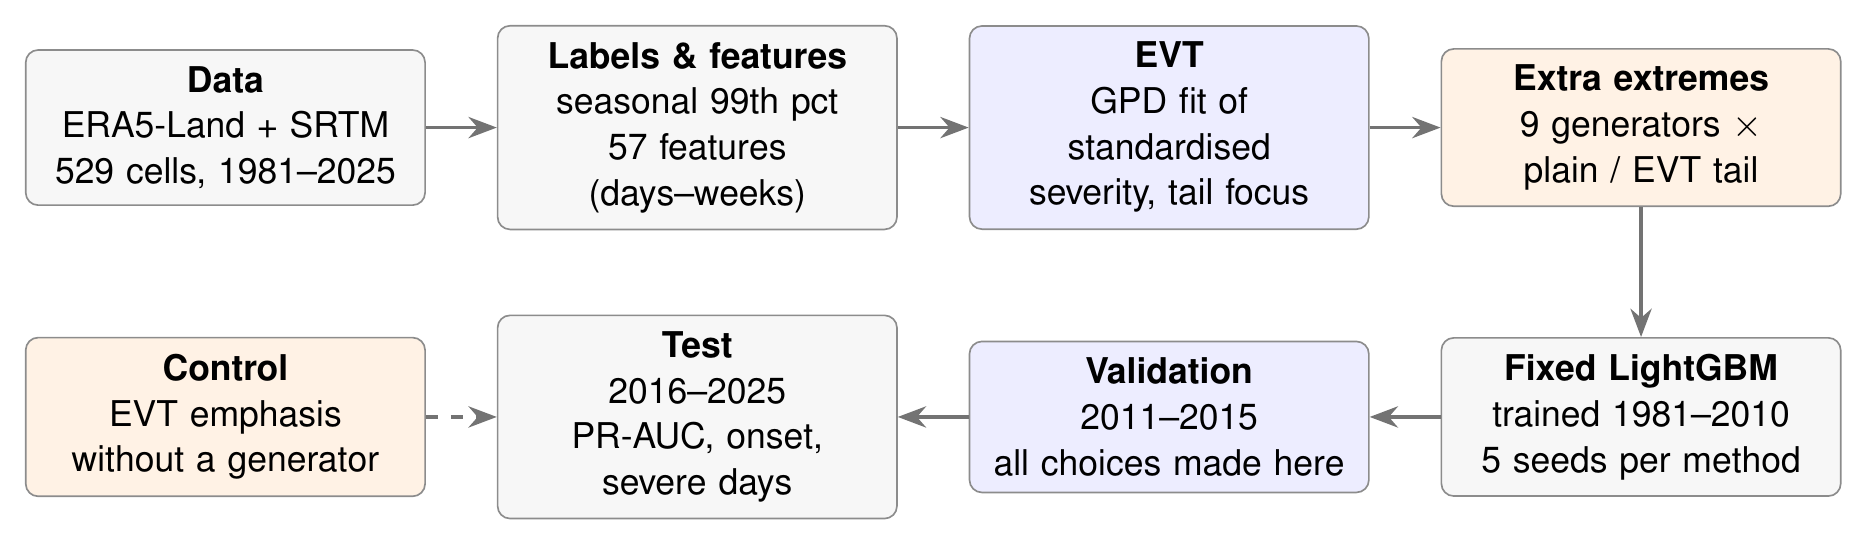
\includegraphics[width=\textwidth]{fig_pipeline.png}
\caption{Overview of the project pipeline}
\label{fig:pipeline}
\end{figure}

\section{Problem Statement}
The project title is \textbf{Extreme Value-Guided Deep Generative Models for Imbalanced Classification}, with four
objectives:
\begin{enumerate}
  \item treat the minority class as a tail phenomenon;
  \item use EVT to characterise and constrain the tail;
  \item use generative models (GANs, diffusion and others) to augment and rebalance the training data;
  \item ensure that the synthetic data are statistically consistent with real extremes, and test whether they
        improve the classifier.
\end{enumerate}
The final research question, agreed with the supervisor, is: \emph{with one fixed classifier (LightGBM) that
predicts next-day extreme heat from the previous days and weeks, which way of generating extra extreme days helps
most, and what does EVT add?}

\section{Beneficiaries (Intended Users)}
\begin{itemize}
  \item \textbf{Disaster management and public-health authorities} in Himachal Pradesh, who need local, next-day
        heat warnings to activate heat action plans.
  \item \textbf{Agriculture and horticulture}, in particular apple growers, for whom unusual heat at a given altitude
        and season matters more than an absolute temperature.
  \item \textbf{Water, hydropower and glacier-melt planners}, who are affected by warm spells in the high mountains.
  \item \textbf{Weather services}, as a light-weight, interpretable statistical layer on top of existing forecasts.
  \item \textbf{Researchers in imbalanced learning}, for whom the framework---EVT to target synthetic data, compared
        under a fixed classifier---applies to any problem in which the rare class is the tail of a distribution
        (fraud, equipment failure, floods).
\end{itemize}

% =============================================================================
\chapter{Market Research}
% =============================================================================
\section{Existing Products and Approaches}
Heat prediction and rare-event classification are served today by several kinds of products and methods.
\begin{itemize}
  \item \textbf{Operational heat-wave warnings (IMD):} The India Meteorological Department declares a heat wave in
        the hills when the maximum temperature is at least 30\,$^\circ$C and exceeds normal by 4.5--6.4\,$^\circ$C
        (a severe heat wave above 6.4\,$^\circ$C), when this holds at two or more stations of a sub-division on two
        consecutive days. It issues colour-coded warnings (green, yellow, orange, red) for about 660 districts with
        a five-day horizon, and city forecasts~\cite{bhan_imd}.
  \item \textbf{Numerical weather prediction (NWP):} physics-based global models such as the ECMWF high-resolution
        forecast simulate the atmosphere on supercomputers. They remain the most reliable source for record
        extremes~\cite{zhang2025records}.
  \item \textbf{AI weather models:} data-driven global models such as GraphCast, Pangu-Weather and FuXi produce fast
        forecasts at about 0.25$^\circ$, but have been shown to under-predict record-breaking heat and other
        extremes~\cite{zhang2025records,lopezgomez2023heat}.
  \item \textbf{Machine-learning classifiers with rebalancing:} gradient-boosted trees or neural networks trained with
        class weights or SMOTE-type oversampling~\cite{chawla2002smote,han2005borderline,he2008adasyn}.
  \item \textbf{Synthetic data tools:} libraries such as the Synthetic Data Vault~\cite{patki2016sdv} provide
        Gaussian copula, CTGAN, TVAE and CopulaGAN generators for tabular data.
\end{itemize}

\section{Comparison with Existing Products/Technologies}
\begin{table}[H]
\centering
\caption{Comparison of existing approaches with the approach of this project}
\label{tab:market}
\footnotesize
\begin{tabularx}{\textwidth}{|>{\centering\arraybackslash}p{2.3cm}|>{\centering\arraybackslash}X|>{\centering\arraybackslash}X|>{\centering\arraybackslash}p{1.8cm}|>{\centering\arraybackslash}X|}
\hline
\textbf{Approach} & \textbf{What is ``extreme''} & \textbf{Handling of rare, severe days} & \textbf{Compute} & \textbf{Limitation for this problem}\\ \hline
IMD warnings & Absolute and departure thresholds at stations & Expert rules, operational & Operational system & Station/sub-division scale; fixed thresholds \\ \hline
NWP (e.g.\ ECMWF) & Any forecast variable & Physics; best for records & Supercomputer & Not available to students; no local extreme label \\ \hline
AI weather models & Any forecast variable & Under-predict records & GPU (inference) & Coarse (0.25$^\circ$); trained for average skill \\ \hline
Classifier + SMOTE / weights & Labels supplied by user & Interpolation or weighting & Low & Little gain for strong classifiers~\cite{elor2022smote} \\ \hline
Generic tabular generators & Labels supplied by user & Learn the bulk of the data & Medium (GPU) & Ignore the tail; often break physics \\ \hline
\textbf{This project} & Per-cell, per-season 99th percentile & EVT tail focus + generators & Free Colab & Next-day, reanalysis-based \\ \hline
\end{tabularx}
\end{table}

\section{Problems with Existing Alternatives}
\begin{itemize}
  \item \textbf{Fixed thresholds do not describe local extremes.} An absolute rule such as 30\,$^\circ$C in the hills
        suits towns, but at high-altitude cells, where the maximum temperature rarely reaches 30\,$^\circ$C, a day can
        be extreme for its own climate without crossing it.
  \item \textbf{Average-skill models miss the tail.} AI weather models trained to minimise average error
        under-predict how often and how strongly records occur~\cite{zhang2025records}.
  \item \textbf{Standard rebalancing gives little.} For strong classifiers such as gradient-boosted trees, balancing
        the classes rarely helps~\cite{elor2022smote}; interpolation cannot reach beyond the most extreme observed
        day.
  \item \textbf{Generic generators are tail-blind.} Generative models learn the bulk of the data; in this project,
        70\% of raw rows from three of them broke simple physical rules.
  \item \textbf{Cost.} NWP and large AI models need resources far beyond a student project.
\end{itemize}

\section{How Our Approach Differs}
\begin{itemize}
  \item \textbf{Local, relative extremes:} every grid cell and season has its own threshold.
  \item \textbf{EVT-guided data:} a fitted extreme value model decides which severities to add, and caps how far
        synthetic severities may go.
  \item \textbf{Generator-independent:} the same EVT tail focus works with interpolation, copulas, VAEs, GANs,
        diffusion---and even with simple copies of real days.
  \item \textbf{Physics by construction} for every synthetic day.
  \item \textbf{Fair, honest comparison:} one fixed classifier, choices on a validation period, five seeds,
        month-block bootstrap tests.
  \item \textbf{Low cost:} everything runs on free cloud resources; the best all-round method needs no generator.
\end{itemize}

% =============================================================================
\chapter{Literature Review}
% =============================================================================
\section{Imbalanced Classification: Overview}
When one class is rare, a classifier that minimises average error can ignore it. Two families of remedies exist.
\emph{Cost-sensitive learning} gives the rare class a larger weight in the loss. \emph{Resampling} changes the
training data: random oversampling copies rare examples, and SMOTE~\cite{chawla2002smote} creates new ones on the
line between a rare example $x_i$ and one of its $k$ nearest rare neighbours $x_{nn}$:
\begin{equation}
  x_{\text{new}} = x_i + \lambda\,(x_{nn}-x_i), \qquad \lambda\sim\mathcal{U}(0,1).
\end{equation}
Borderline-SMOTE~\cite{han2005borderline} generates only near the class boundary, and ADASYN~\cite{he2008adasyn}
generates more where rare examples are hard to learn. A large study by Elor and Averbuch-Elor~\cite{elor2022smote}
found that such balancing seldom improves strong classifiers such as gradient-boosted trees, which matches our
results.

\section{Extreme Value Theory}
EVT~\cite{coles2001} describes the behaviour of a variable far out in its tail. In the \emph{peaks-over-threshold}
(POT) approach, the Pickands--Balkema--de Haan theorem~\cite{pickands1975,balkema1974} states that for a high
threshold $u$, the excess $Y=X-u$ given $X>u$ is approximately Generalized Pareto distributed:
\begin{equation}
  F_{\xi,\sigma}(y)=1-\left(1+\frac{\xi y}{\sigma}\right)^{-1/\xi},\qquad y>0,\; 1+\frac{\xi y}{\sigma}>0 .
  \label{eq:gpd}
\end{equation}
The scale $\sigma>0$ sets the spread of excesses and the shape $\xi$ the type of tail: $\xi<0$ gives a bounded tail
with upper end point $u+\sigma/|\xi|$ (expected for temperature), $\xi=0$ an exponential tail, and $\xi>0$ a heavy
tail. Parameters are estimated by maximum likelihood,
\begin{equation}
  \hat\xi,\hat\sigma=\arg\max_{\xi,\sigma}\sum_{i=1}^{n}\left[-\log\sigma-\left(1+\frac{1}{\xi}\right)
  \log\left(1+\frac{\xi y_i}{\sigma}\right)\right].
\end{equation}

\section{Deep Generative Models for Tabular Data}
\subsection{Generative adversarial networks}
A GAN~\cite{goodfellow2014gan} trains a generator $G$ to turn random noise $z$ into samples that a discriminator $D$
cannot tell from real data:
\begin{equation}
  \min_G\max_D\; \mathbb{E}_{x\sim p_{\text{data}}}[\log D(x)]+\mathbb{E}_{z\sim p_z}[\log(1-D(G(z)))].
\end{equation}
The Wasserstein GAN with gradient penalty (WGAN-GP)~\cite{gulrajani2017wgangp} replaces the discriminator by a critic
$D$ and stabilises training with
\begin{equation}
  \mathcal{L}_D=\mathbb{E}[D(G(z))]-\mathbb{E}[D(x)]+\lambda\,\mathbb{E}_{\hat x}\left[\left(\lVert\nabla_{\hat x}D(\hat x)\rVert_2-1\right)^2\right],
\end{equation}
where $\hat x$ are random points between real and generated samples. CTGAN~\cite{xu2019ctgan} adapts GANs to tables
with mode-specific normalisation of numerical columns and a conditional vector for categorical columns; CopulaGAN
first transforms each column through its fitted marginal distribution.

\subsection{Variational autoencoders and copulas}
A VAE~\cite{kingma2014vae} encodes a sample $x$ into a latent variable $z$ and decodes it back, maximising the
evidence lower bound
\begin{equation}
  \mathcal{L}=\mathbb{E}_{q_\phi(z|x)}[\log p_\theta(x|z)]-\mathrm{KL}\left(q_\phi(z|x)\,\Vert\,p(z)\right).
\end{equation}
TVAE~\cite{xu2019ctgan} is its tabular version. A Gaussian copula~\cite{patki2016sdv} models each column's marginal
distribution separately and their dependence through a multivariate normal correlation matrix.

\subsection{Diffusion models}
Denoising diffusion models~\cite{ho2020ddpm} gradually add Gaussian noise to the data over $T$ steps,
\begin{equation}
  q(x_\tau\mid x_0)=\mathcal{N}\!\left(\sqrt{\bar\alpha_\tau}\,x_0,\,(1-\bar\alpha_\tau)I\right),
\end{equation}
and train a network $\epsilon_\theta$ to predict the added noise,
\begin{equation}
  \mathcal{L}=\mathbb{E}_{x_0,\tau,\epsilon}\left\lVert\epsilon-\epsilon_\theta\!\left(\sqrt{\bar\alpha_\tau}x_0+\sqrt{1-\bar\alpha_\tau}\,\epsilon,\;\tau,\;c\right)\right\rVert^2 .
\end{equation}
New samples are produced by reversing the process, here with fast DDIM sampling~\cite{song2021ddim} and a cosine
noise schedule~\cite{nichol2021improved}. With classifier-free guidance~\cite{ho2022cfg} the condition $c$ is
strengthened by
\begin{equation}
  \hat\epsilon=(1+w)\,\epsilon_\theta(x,\tau,c)-w\,\epsilon_\theta(x,\tau,\varnothing).
\end{equation}
TabDDPM~\cite{kotelnikov2023tabddpm} showed that diffusion models are strong generators for tabular data, and
D'souza et al.~\cite{dsouza2025overlap} that they produce better minority samples than GANs.

\section{Extremes, Generative Models and Weather}
Several works connect generative models with extremes. ExGAN~\cite{bhatia2021exgan} generates samples of a chosen
extremeness; evtGAN~\cite{boulaguiem2022evtgan} combines EVT margins with GANs to simulate spatial weather extremes;
heavy-tailed diffusion models~\cite{pandey2025heavy} change the noise distribution to reach far tails; and Jalalzai et
al.~\cite{jalalzai2018extreme} study classification in extreme regions of the input space. For heat forecasting,
neural weather models under-predict the most extreme events~\cite{lopezgomez2023heat}, and numerical models beat AI
models on record-breaking extremes~\cite{zhang2025records}.

\section{Challenges in Existing Models}
\begin{itemize}
  \item Generative models are trained to reproduce the bulk of the data, so the rarest severities are
        under-represented, and tabular generators do not respect physical relations between columns.
  \item EVT-based generators are designed to \emph{simulate} extremes; whether their output improves a downstream
        classifier is rarely tested.
  \item Comparisons of oversampling methods often use one classifier run, although results on rare classes vary
        strongly with training randomness.
\end{itemize}

\section{Significance to the Present Study}
This project uses EVT not to replace the generator but to \emph{guide} it: the fitted Generalized Pareto
Distribution decides which severities are requested or selected. Because this guidance is independent of the
generator, the same EVT tail focus can be applied to interpolation, copulas, VAEs, GANs, diffusion, and plain copies
of real days, and compared fairly under one fixed classifier.

% =============================================================================
\chapter{Data and Methodology}
% =============================================================================
\section{Study Area and Data Sources}
Himachal Pradesh rises from about 300\,m in the south-western foothills to more than 5\,km in the north-east.
The study uses all 529 ERA5-Land grid cells (0.1$^\circ$, about 10\,km) whose centre lies in the state
(Figure~\ref{fig:area}); the data sources are listed in Table~\ref{tab:sources}.

\begin{figure}[H]
\centering
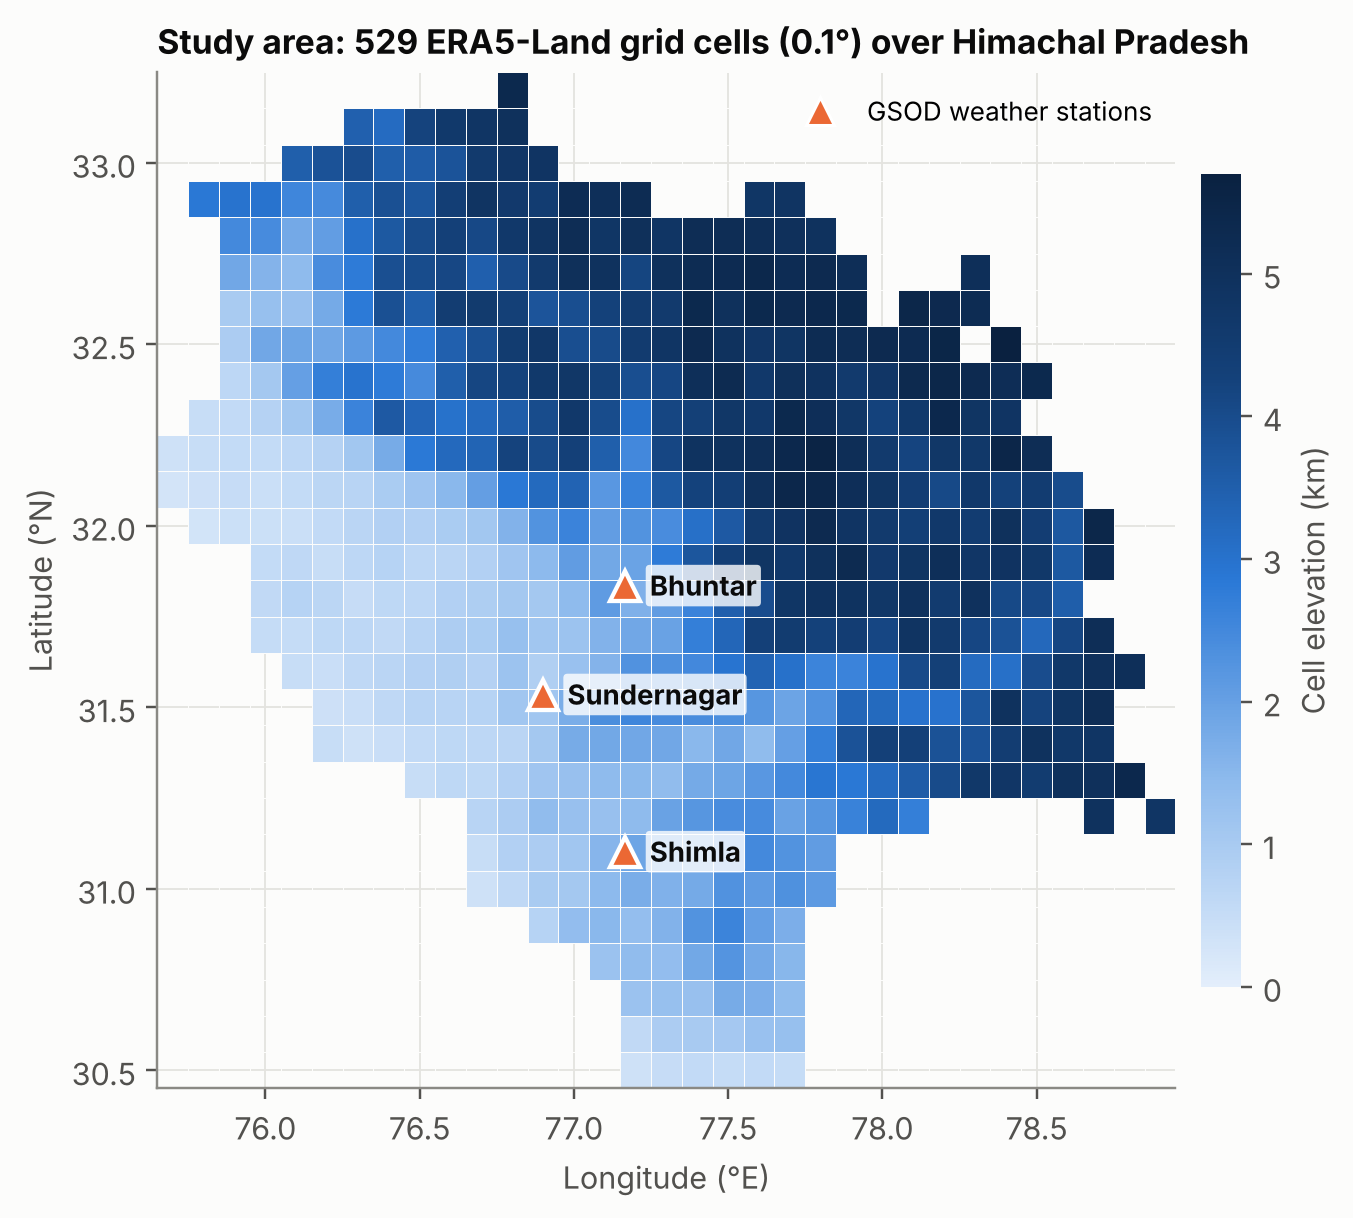
\includegraphics[width=0.82\textwidth]{fig_study_area.png}
\caption{Study area: 529 ERA5-Land grid cells coloured by elevation, and the three GSOD stations}
\label{fig:area}
\end{figure}

\begin{table}[H]
\centering
\caption{Data sources used in the project}
\label{tab:sources}
\small
\begin{tabularx}{\textwidth}{|p{3.0cm}|X|p{3.2cm}|p{2.6cm}|}
\hline
\textbf{Source} & \textbf{Variables} & \textbf{Period, resolution} & \textbf{Role}\\ \hline
ERA5-Land~\cite{munoz2021era5land} & Daily maximum, minimum and mean temperature, dewpoint, relative humidity, surface pressure, solar radiation, soil moisture, precipitation & 1981--2025, 0.1$^\circ$ & Labels and features \\ \hline
SRTM~\cite{farr2007srtm} & Elevation, slope & 30\,m, averaged to cells & Terrain features \\ \hline
GADM boundary & State outline & -- & Cell mask \\ \hline
IMD gridded data & Maximum and minimum temperature & 1981--2025, 1$^\circ$ & Regional check \\ \hline
NOAA GSOD & Station temperature (Shimla, Sundernagar, Bhuntar) & 2016--2025 & Reference stations \\ \hline
\end{tabularx}
\end{table}

ERA5-Land is the only data set that is complete for 45 years at a resolution fine enough for mountainous terrain.
It has absolute biases on steep slopes, but our labels compare each cell with its own history, so a constant bias
shifts the threshold and not the set of extreme days.

\section{Pre-processing and Verification}
\begin{itemize}
  \item All inputs were placed on the ERA5-Land grid (30.3--33.3$^\circ$N, 75.5--79.1$^\circ$E), masked to the state,
        giving 529 cells and 16{,}436 days.
  \item Temperatures were converted from kelvin to $^\circ$C, pressure to hPa, radiation to W\,m$^{-2}$ and
        precipitation to mm; accumulated variables were shifted back by the one day by which ERA5-Land stamps them.
  \item The processed file was verified against the raw files for five cells (522--5{,}279\,m) and six years: all
        variables match after unit conversion, and no day has $T_{\min}>T_{\max}$.
  \item Missing mean temperature and humidity for 1981--1985 were refilled from the raw files.
  \item IMD data stored missing values as 99.9 and $-999$; these codes were treated as missing, not as
        temperatures.
\end{itemize}

\section{Defining Extreme Heat Days}
For cell $c$, day $t$ and season $g$ (winter Dec--Feb, pre-monsoon Mar--May, monsoon Jun--Sep, post-monsoon Oct--Nov),
the threshold $u_{c,g}$ is the 99th percentile of the daily maximum temperature $T^{\max}$ over the days of season $g$
in the base period 1981--2010. Day $t$ is an extreme heat day if
\begin{equation}
  y_{c,t}=\mathbb{1}\!\left[T^{\max}_{c,t}>u_{c,g(t)}\right].
\end{equation}
Thresholds fall by about 6--7\,$^\circ$C per kilometre of altitude (Figure~\ref{fig:thr}), consistent with the
atmospheric lapse rate.

\begin{figure}[H]
\centering
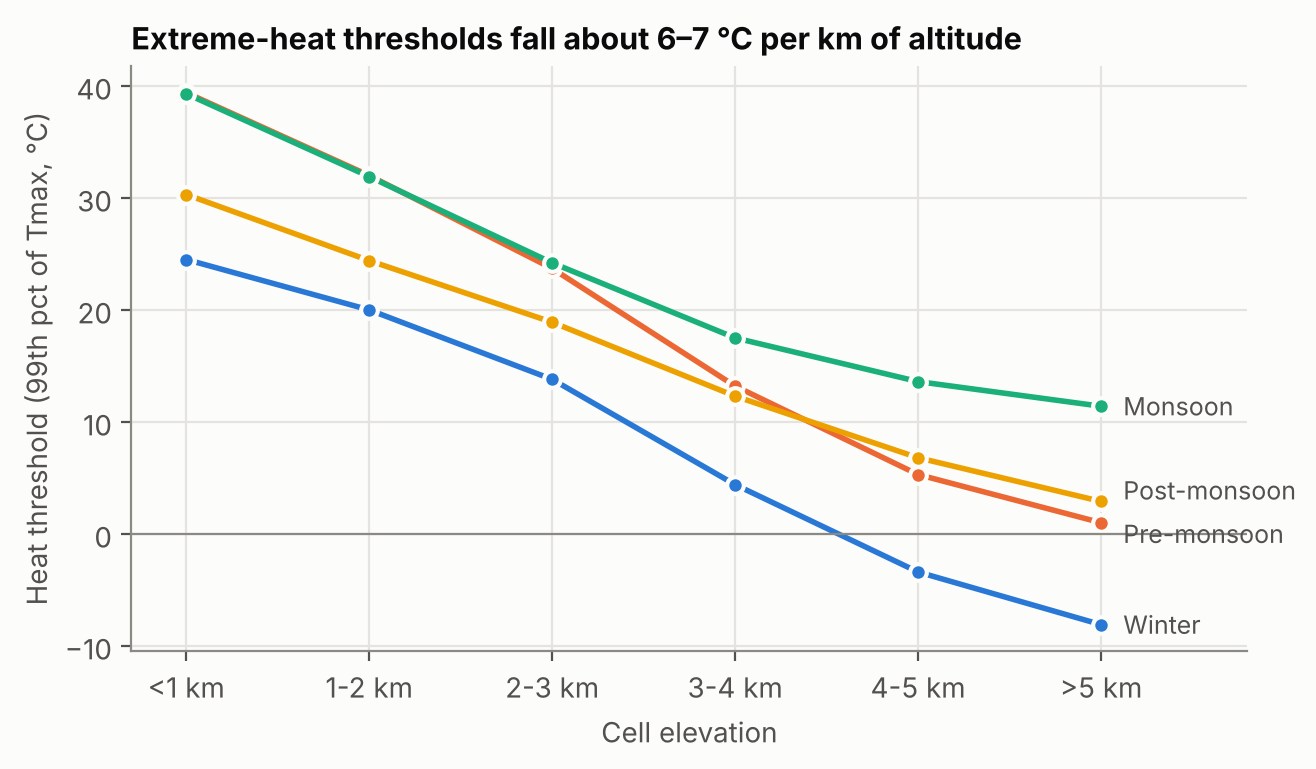
\includegraphics[width=0.82\textwidth]{fig_thresholds.png}
\caption{Mean extreme-heat threshold by elevation band and season (1981--2010)}
\label{fig:thr}
\end{figure}

The labels show four clear patterns:
\begin{itemize}
  \item \textbf{Warming:} heat extremes nearly doubled in 2016--2025 (1.94\% of cell-days against 1.02\% in
        1981--2010); 2024 had the most widespread heat.
  \item \textbf{Strongest signal in October--November:} post-monsoon heat extremes reached 11.0\% of days in 2020
        and 6--7\% in 2017, 2021 and 2024, against a 1\% baseline.
  \item \textbf{Clustering:} on 6 October 1983, 522 of the 529 cells were extreme at once; training positives come
        from a few hundred events.
  \item \textbf{Season edges:} seasonal extremes gather at the warm edge of each season (May, early October).
\end{itemize}

\section{Prediction Task, Features and Data Splits}
Each sample is one cell on day $t$; the target is whether day $t+1$ is an extreme heat day. Only information
available on day $t$ is used (Table~\ref{tab:features}). The data are split by year, because neighbouring days and
cells are strongly correlated (Table~\ref{tab:splits}).

\begin{table}[H]
\centering
\caption{The 57 input features}
\label{tab:features}
\small
\begin{tabularx}{\textwidth}{|p{3.6cm}|X|}
\hline
\textbf{Group} & \textbf{Features}\\ \hline
Terrain (4) & Latitude, longitude, elevation, slope \\ \hline
Recent weather (29) & Maximum, minimum and mean temperature, dewpoint, relative humidity, pressure, solar radiation, soil moisture and precipitation on days $t$, $t-1$, $t-2$; today's maximum and minimum temperature anomaly \\ \hline
Longer history (16) & Mean maximum-temperature anomaly over 7, 14, 30 days; minimum-temperature anomaly over 7, 30 days; length of the current warm spell; days since the last extreme; extremes in the last 30 days; rain over 7 and 30 days; soil moisture over 14 and 30 days and its 14-day change; 7-day dewpoint and radiation; 3-day pressure change \\ \hline
Distance to threshold (8) & Today's, yesterday's and the day before's maximum temperature minus tomorrow's threshold, in $^\circ$C and in units of the cell's variability; their trend; day-to-day change \\ \hline
\end{tabularx}
\end{table}

\begin{table}[H]
\centering
\caption{Training, validation and test splits}
\label{tab:splits}
\small
\begin{tabular}{|l|c|l|r|r|r|}
\hline
\textbf{Split} & \textbf{Years} & \textbf{Used for} & \textbf{Rows} & \textbf{Extremes} & \textbf{Share}\\ \hline
Train (random half) & 1981--2010 & Fitting all models & 2{,}889{,}927 & 29{,}604 & 1.02\% \\ \hline
Validation & 2011--2015 & Every choice & 965{,}954 & 9{,}626 & 1.00\% \\ \hline
Test & 2016--2025 & Final scores only & 1{,}932{,}437 & 37{,}450 & 1.94\% \\ \hline
\end{tabular}
\end{table}

Calendar features were deliberately excluded: in a first version the model relied on the day of the year, which
does not transfer to a warmer test decade.

\section{Extreme Value Model of the Minority Class}
Pooling raw excesses from all cells mixes low cells with small day-to-day variability and high cells with large
variability; the mixture looks heavy-tailed even when each cell's tail is bounded. Each excess is therefore
standardised by the cell's own variability $s_{c,g}$ (the standard deviation of its daily temperature anomaly in that
season, 1981--2010):
\begin{equation}
  z_{c,t}=\frac{T^{\max}_{c,t}-u_{c,g(t)}}{s_{c,g(t)}} .
\end{equation}
The severity $z$ is what the GPD (Eq.~\ref{eq:gpd}) describes and what guides the generators; it is never a classifier
input, since it encodes tomorrow's outcome. Parameters were fitted by maximum likelihood on 1981--2010 exceedances,
with 95\% intervals from a bootstrap that resamples whole days.

\begin{table}[H]
\centering
\caption{GPD shape $\xi$ of heat excesses, and the share of 2016--2025 extremes beyond the fitted 90th percentile (0.10 = unchanged tail)}
\label{tab:gpd}
\small
\begin{tabular}{|l|c|c|c|c|}
\hline
\textbf{Group} & \textbf{$\xi$ raw} & \textbf{$\xi$ standardised} & \textbf{95\% interval} & \textbf{Recent beyond q90}\\ \hline
Whole year & $-0.153$ & $-0.152$ & $[-0.196,-0.113]$ & 0.077 \\ \hline
Monsoon & $-0.128$ & $-0.115$ & $[-0.185,-0.040]$ & 0.080 \\ \hline
Pre-monsoon & $-0.165$ & $-0.141$ & $[-0.241,-0.072]$ & 0.103 \\ \hline
Winter & $-0.074$ & $-0.096$ & $[-0.176,-0.032]$ & \textbf{0.209} \\ \hline
Post-monsoon & $0.262$ & $0.070$ & $[-0.177,0.231]$ & 0.063 \\ \hline
\end{tabular}
\end{table}

\begin{figure}[H]
\centering
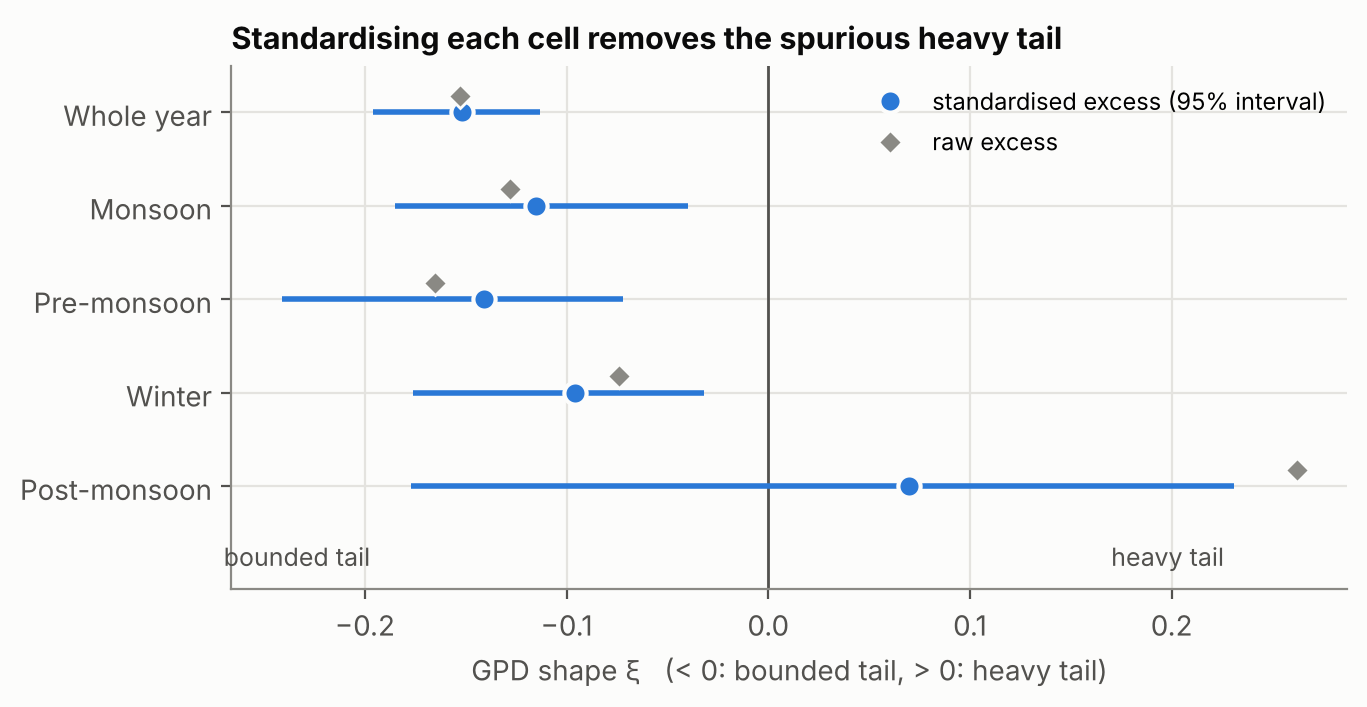
\includegraphics[width=0.82\textwidth]{fig_gpd_shape.png}
\caption{GPD shape parameter for raw and standardised heat excesses}
\label{fig:gpdshape}
\end{figure}

After standardisation every heat tail is bounded or close to it (Table~\ref{tab:gpd}, Figures~\ref{fig:gpdshape}
and~\ref{fig:qq}): the spurious heavy tail of post-monsoon heat largely disappears. Recent winter extremes exceed
the old tail's 90th percentile twice as often as expected, so winter warm spells have become more intense.

\begin{figure}[H]
\centering
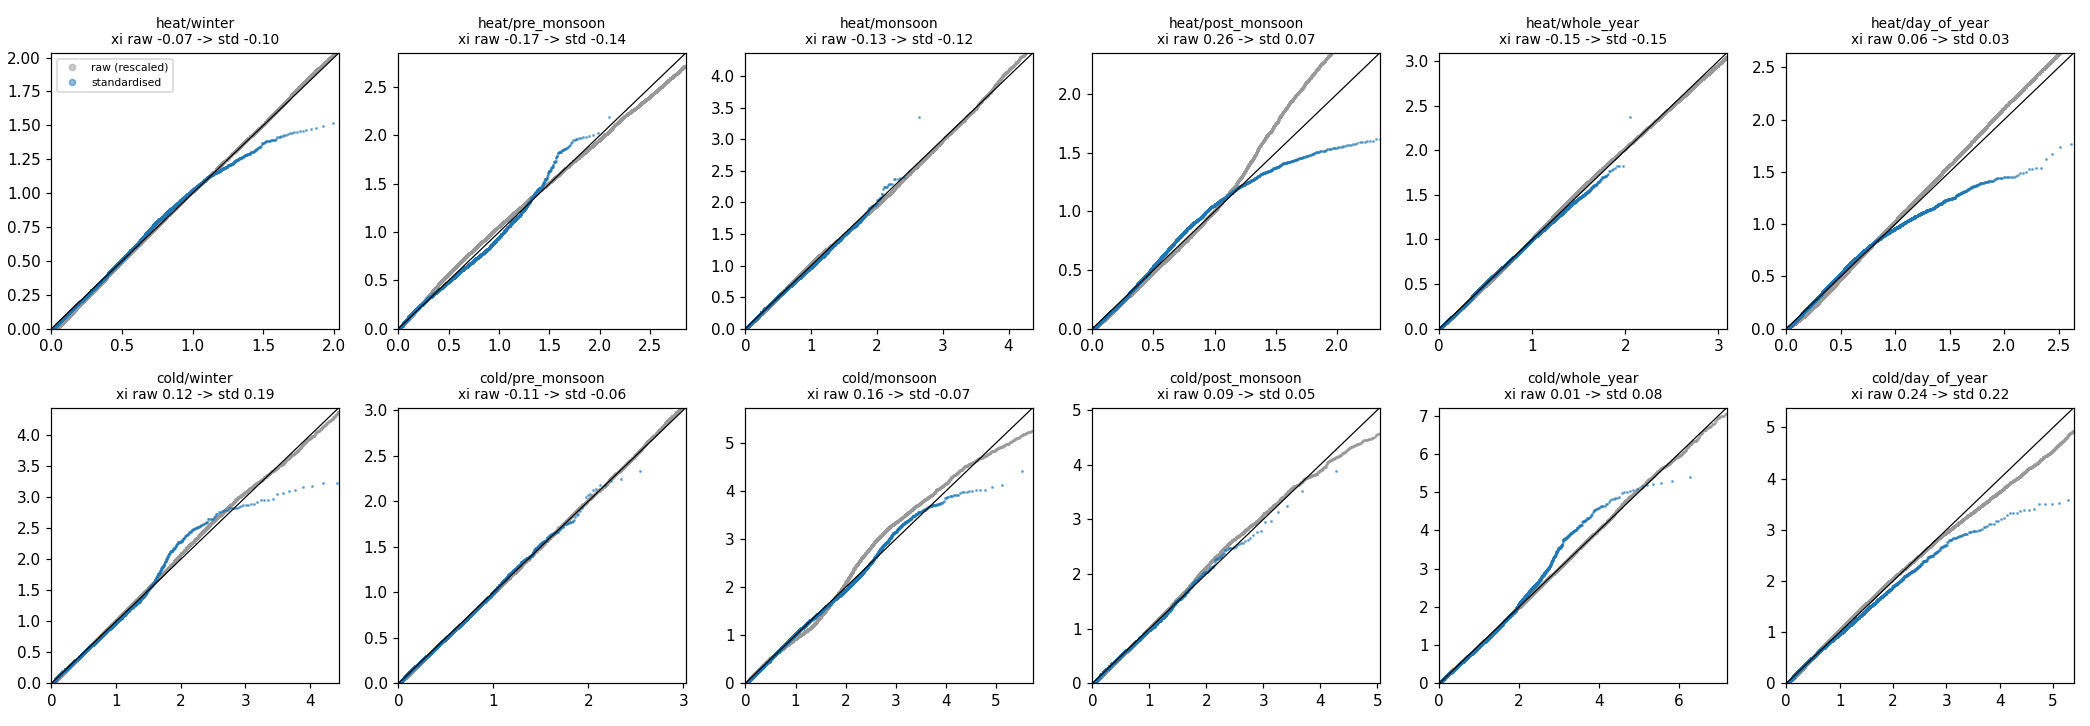
\includegraphics[width=\textwidth]{evt_qq_std.png}
\caption{GPD quantile--quantile plots of raw (grey) and standardised (blue) excesses, 1981--2010}
\label{fig:qq}
\end{figure}

\section{EVT Tail Focus}
The fitted GPD gives every extreme a \emph{tail position} $q=F_{\hat\xi,\hat\sigma}(z)\in[0,1)$ within its season;
$q=0.9$ means that only 10\% of extremes are more severe. Real extremes are spread evenly over $q$. EVT tail focus
draws the tail positions of the added extremes from
\begin{equation}
  q\sim 0.5\,\mathcal{U}(0,1)+0.5\,\mathcal{U}(0.8,1),
\end{equation}
so that 60\% of them lie in the top 20\% of the tail (Figure~\ref{fig:tailfocus}). Severities are obtained from the
GPD quantile function and capped at the tail's end point and at 1.5 times the largest observed severity of the
season, so EVT may extrapolate moderately but not without limit.

\begin{figure}[H]
\centering
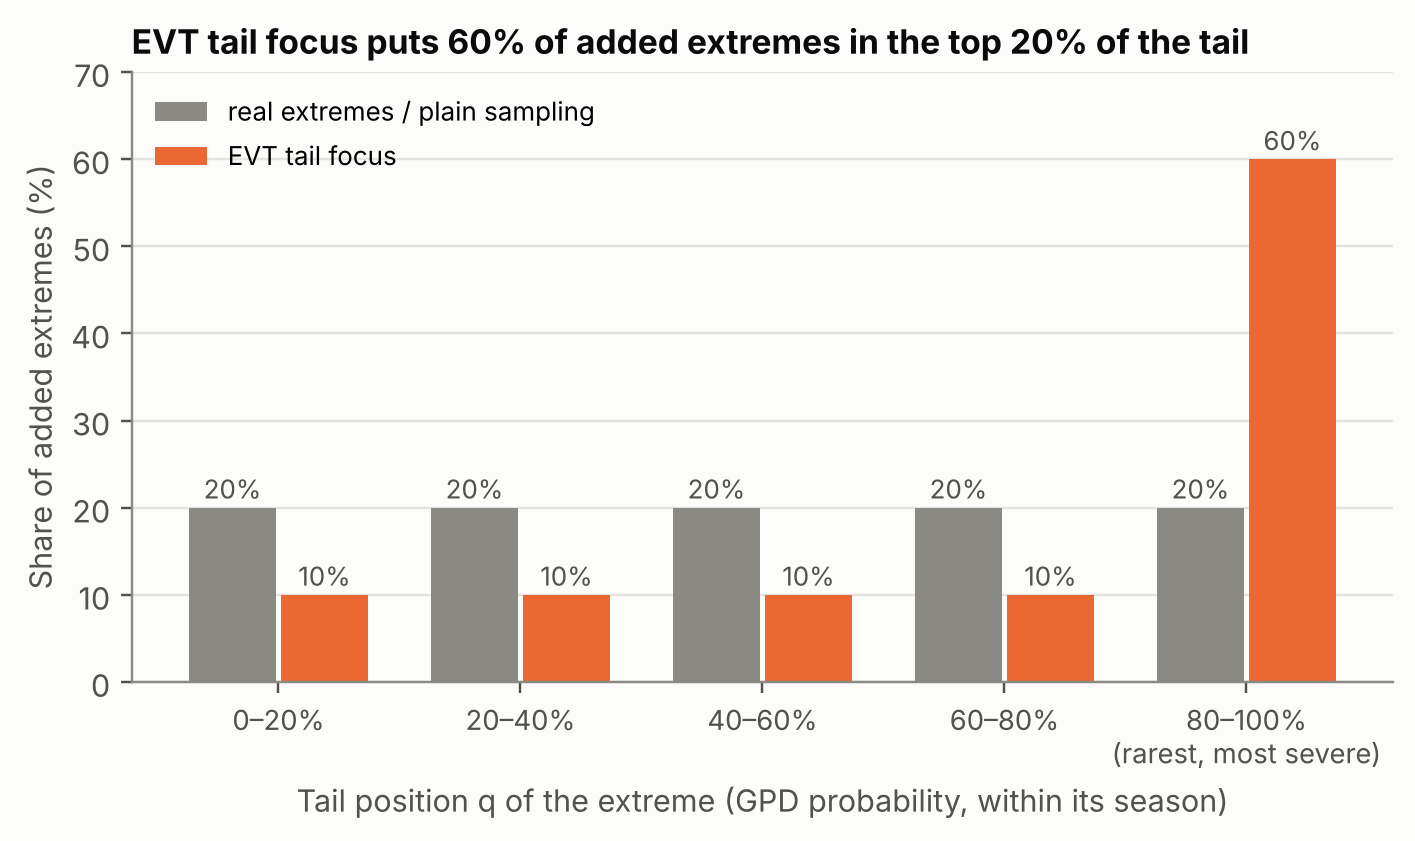
\includegraphics[width=0.82\textwidth]{fig_tail_focus.png}
\caption{Distribution of the added extremes over the tail: plain sampling versus EVT tail focus}
\label{fig:tailfocus}
\end{figure}

\section{Generation Methods}
Table~\ref{tab:methods} lists the methods compared. Each method adds exactly one synthetic extreme per real
extreme (29{,}604 rows), drawn again for every training seed; each generator is used \emph{plain} and with
\emph{EVT tail focus}.

\begin{table}[H]
\centering
\caption{Generation methods and how EVT tail focus is applied}
\label{tab:methods}
\small
\begin{tabularx}{\textwidth}{|p{3.3cm}|p{2.2cm}|p{2.6cm}|X|}
\hline
\textbf{Method} & \textbf{Family} & \textbf{EVT tail focus} & \textbf{Description}\\ \hline
SMOTE~\cite{chawla2002smote} & Interpolation & -- & Points between real extremes and their neighbours \\ \hline
Borderline-SMOTE~\cite{han2005borderline} & Interpolation & -- & Only near the class boundary \\ \hline
ADASYN~\cite{he2008adasyn} & Interpolation & -- & More where extremes are hard to learn \\ \hline
Gaussian copula~\cite{patki2016sdv} & Statistical & Selection & Column margins plus a correlation structure \\ \hline
TVAE~\cite{xu2019ctgan} & VAE & Selection & Tabular variational autoencoder \\ \hline
CTGAN~\cite{xu2019ctgan} & GAN & Selection & Conditional tabular GAN \\ \hline
CopulaGAN~\cite{patki2016sdv} & GAN & Selection & CTGAN on copula-transformed columns \\ \hline
Conditional WGAN-GP~\cite{gulrajani2017wgangp} & GAN & Requested & Designed here; takes season and severity as input \\ \hline
Conditional diffusion & Diffusion & Requested & Designed here; takes season and severity as input \\ \hline
Random / EVT-tail copies & None & Selection & Copies of real extremes (control) \\ \hline
EVT-tail weights & None & Weighting & Extra training weight on real extremes (control) \\ \hline
\end{tabularx}
\end{table}

\subsection{Conditional diffusion model}
A denoising diffusion model was trained on the 29{,}604 real training extremes, modelling the 49 base features
after a quantile transform to a standard normal per feature. The denoiser is a residual multi-layer perceptron
(width 512, four blocks) with a time embedding and the condition $c=[\text{season},\,z/0.5,\,1]$, which is set to
zero for 10\% of training rows. It was trained for 15{,}000 steps (batch 1{,}024, AdamW, exponential moving average
of the weights; about 30 minutes on a free T4 GPU) with $T=1000$ steps, and sampled with 50 DDIM steps and guidance
weight $w=2$.

\subsection{Conditional WGAN-GP}
Generator and critic are three-layer MLPs of width 512, conditioned on the same input as the diffusion model; the
gradient penalty weight is 10, with five critic updates per generator update and 6{,}000 generator updates
(about 3 minutes on a T4).

\subsection{Unconditional generators and EVT selection}
Gaussian copula, TVAE, CTGAN and CopulaGAN (SDV 2.2 defaults: 300 epochs, batch 500) cannot be told a severity.
For these, EVT tail focus is applied by selection:
\begin{enumerate}
  \item generate a pool ten times larger than needed (296{,}040 rows);
  \item score each row with a severity ``judge'' (a LightGBM regressor trained on real extremes; Spearman correlation
        0.769 on unseen real extremes) and convert the judged severity to a tail position $q$;
  \item select rows so that $q$ follows the tail-focus target, keeping the real share of each season.
\end{enumerate}

\subsection{Physics by construction}
Every synthetic row from every generator is snapped to the nearest real grid cell (which fixes terrain, threshold
and variability); the minimum, mean and maximum temperatures of each day are sorted; humidity, rain, radiation and
soil moisture are clipped to physical ranges; and the distance-to-threshold features are recomputed exactly.

\section{Classifier and Evaluation Protocol}
\subsection{Classifier}
The classifier is LightGBM~\cite{ke2017lightgbm}, a gradient-boosted decision tree ensemble
$\hat f(x)=\sum_{m=1}^{M} f_m(x)$, with learning rate 0.05, 31 leaves, at least 200 rows per leaf, up to 1{,}000 trees
with early stopping on validation PR-AUC, and a monotone constraint that a larger distance to tomorrow's threshold
can only increase the predicted risk. It is identical for every method.

\subsection{Scores}
Because extreme days are rare, accuracy is uninformative (a model that never warns is 98\% accurate). We use the area
under the precision--recall curve (PR-AUC), computed as average precision,
\begin{equation}
  \mathrm{AP}=\sum_{k}\left(R_k-R_{k-1}\right)P_k ,
\end{equation}
where $P_k$ and $R_k$ are precision and recall at the $k$-th threshold. A random classifier scores 0.019 on the test
decade. Three versions are reported:
\begin{itemize}
  \item \textbf{PR-AUC} on all test days;
  \item \textbf{onset PR-AUC} on days where today is not yet above tomorrow's threshold (heatwave starts);
  \item \textbf{severe PR-AUC}: normal days against the 10\% most severe test extremes (3{,}745 cell-days).
\end{itemize}
At the F1-optimal threshold chosen on validation we also report precision, recall and the critical success index
\begin{equation}
  \mathrm{CSI}=\frac{\mathrm{TP}}{\mathrm{TP}+\mathrm{FP}+\mathrm{FN}} .
\end{equation}

\subsection{Baseline, uncertainty and selection}
\begin{itemize}
  \item \textbf{Persistence baseline:} the score is today's distance to tomorrow's threshold, i.e.\ ``tomorrow will
        be like today''. It is strong because heat persists.
  \item \textbf{Five seeds:} every method is trained with five seeds, which change LightGBM's randomness and which
        synthetic rows are drawn; \emph{seed-averaged} models average the five predicted probabilities.
  \item \textbf{Month-block bootstrap:} 95\% intervals and paired comparisons resample whole test months
        (200 times); a share of resamples $\ge0.95$ in which one model is better is read as a convincing win.
  \item \textbf{Validation-only choices:} the amount of synthetic data, thresholds and the final model are chosen on
        2011--2015; the test decade is used only for scoring.
\end{itemize}

% =============================================================================
\chapter{Results and Discussion}
% =============================================================================
\section{Building an EVT-Guided Generator}
\subsection{First comparison and the amount of synthetic data}
A first comparison with 8.7 synthetic rows per real extreme and one seed (Table~\ref{tab:step8}) showed that plain
LightGBM is much weaker than persistence on the most severe extremes (0.461 against 0.565), that large amounts of
synthetic data lower onset skill, and that every synthetic set hurt a neural-network (MLP) classifier. LightGBM was
therefore kept as the classifier. Varying the amount of synthetic data (Figure~\ref{fig:ratio}) showed that one
synthetic extreme per real extreme works best; this amount is used from here on.

\begin{table}[H]
\centering
\caption{First comparison: test results (2016--2025), one seed, 8.7 synthetic rows per real extreme}
\label{tab:step8}
\small
\begin{tabular}{|l|l|c|c|c|c|c|c|}
\hline
\textbf{Classifier} & \textbf{Training data} & \textbf{PR-AUC} & \textbf{Onset} & \textbf{Severe} & \textbf{Precision} & \textbf{Recall} & \textbf{CSI}\\ \hline
-- & Persistence & 0.586 & 0.191 & 0.565 & 0.553 & 0.602 & 0.405 \\ \hline
\multirow{7}{*}{LightGBM} & Real only & \textbf{0.594} & \textbf{0.227} & 0.461 & 0.623 & 0.518 & 0.394 \\
 & Class weights & 0.590 & 0.219 & 0.443 & 0.622 & 0.535 & 0.404 \\
 & SMOTE & 0.579 & 0.207 & 0.410 & 0.563 & 0.580 & 0.400 \\
 & CTGAN & 0.523 & 0.122 & 0.422 & 0.548 & 0.489 & 0.348 \\
 & Diffusion, no EVT & 0.578 & 0.195 & 0.455 & 0.578 & 0.578 & 0.407 \\
 & Diffusion, EVT & 0.585 & 0.182 & \textbf{0.580} & 0.565 & 0.584 & 0.403 \\
 & Diffusion, EVT tail & 0.589 & 0.189 & 0.563 & 0.563 & 0.598 & 0.408 \\ \hline
\multirow{3}{*}{MLP} & Real only & \textbf{0.597} & \textbf{0.240} & 0.576 & 0.575 & 0.571 & 0.402 \\
 & Class weights & 0.592 & 0.231 & \textbf{0.601} & 0.564 & 0.569 & 0.395 \\
 & Diffusion, EVT tail & 0.537 & 0.175 & 0.515 & 0.563 & 0.485 & 0.353 \\ \hline
\end{tabular}
\end{table}

\begin{figure}[H]
\centering
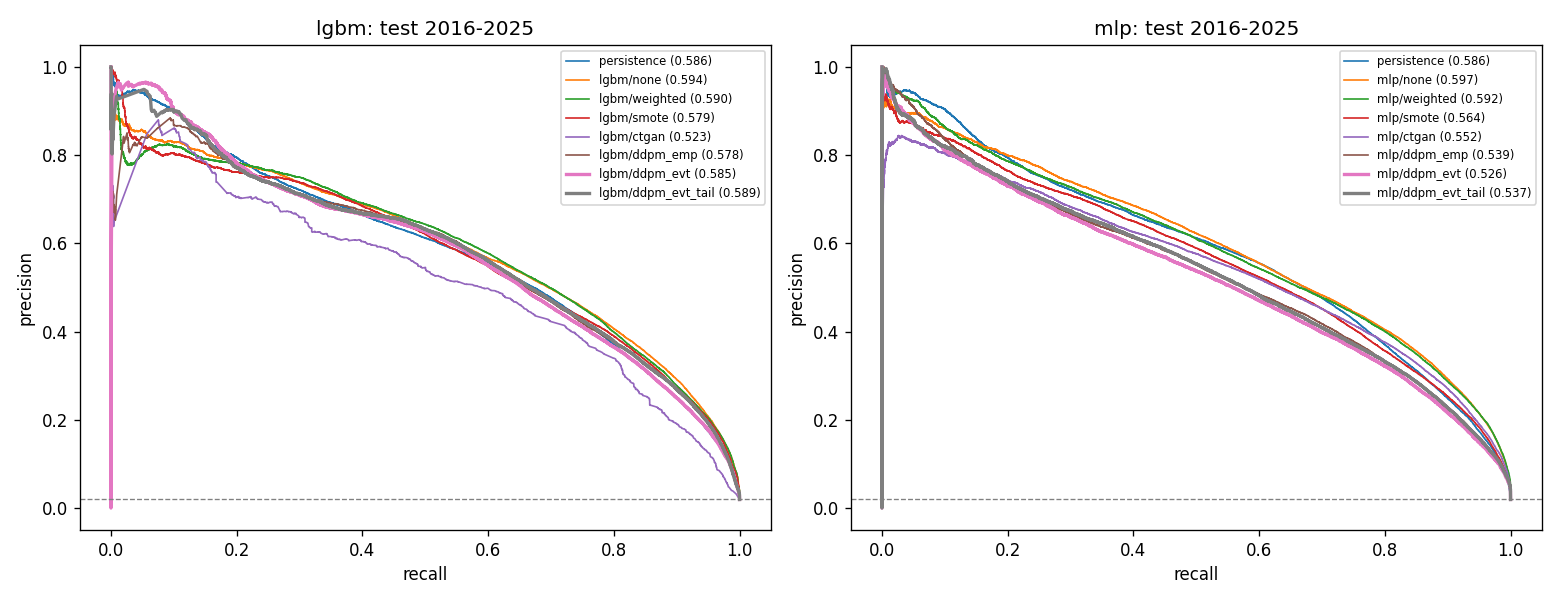
\includegraphics[width=\textwidth]{pr_curves.png}
\caption{Precision--recall curves of the first comparison (one seed)}
\label{fig:pr}
\end{figure}

\begin{figure}[H]
\centering
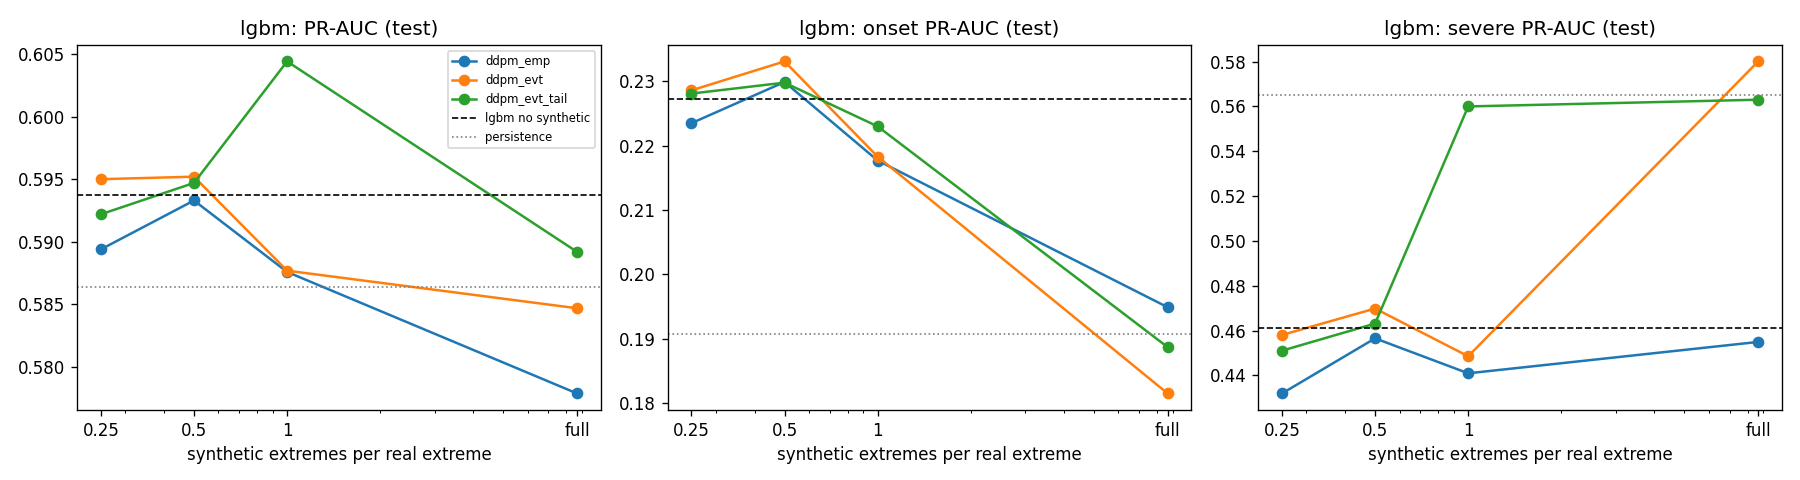
\includegraphics[width=\textwidth]{ratio_sweep.png}
\caption{LightGBM test scores against the number of synthetic extremes per real extreme}
\label{fig:ratio}
\end{figure}

\subsection{Five training seeds}
A one-seed result proved unreliable: the gain of plain EVT over no-EVT diffusion on severe days was $+0.125$,
$-0.057$ and $-0.007$ for three seeds. Every setting was therefore trained with five seeds
(Figure~\ref{fig:seeds}). The robust result is that \emph{EVT tail focus} beats the same diffusion model without
EVT on severe days in all five seeds ($+0.066$), while drawing severities from the fitted GPD as it is gives no gain,
because a well-fitted GPD reproduces almost the same severities as the data.

\begin{figure}[H]
\centering
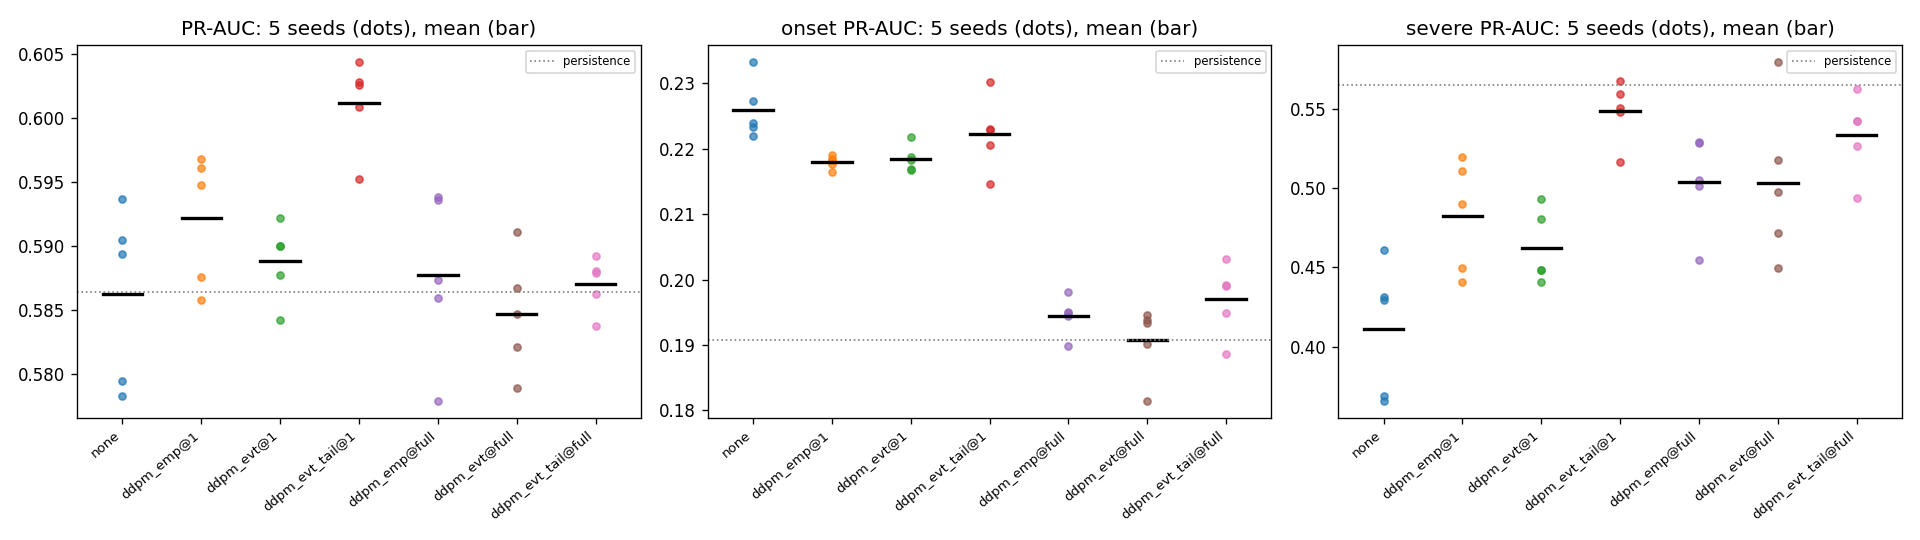
\includegraphics[width=\textwidth]{seed_spread.png}
\caption{Diffusion data with and without EVT: test scores of five seeds per setting}
\label{fig:seeds}
\end{figure}

\section{Properties of the Generators}
\begin{table}[H]
\centering
\caption{Generator properties before any classifier (``top 5\%'': share of output judged in the top 5\% of the tail; real data: 5\%)}
\label{tab:genstats}
\small
\begin{tabular}{|l|c|c|c|c|}
\hline
\textbf{Generator} & \makecell{\textbf{Raw rows}\\\textbf{breaking physics}} & \makecell{\textbf{Top 5\%}\\\textbf{of tail}} & \makecell{\textbf{Follows requested}\\\textbf{severity}} & \makecell{\textbf{Training}\\\textbf{time}} \\ \hline
Gaussian copula & 12.3\% & 18.1\% & -- & 1.8 min \\ \hline
TVAE & 74.7\% & 16.7\% & -- & 18.5 min \\ \hline
CTGAN & 68.7\% & 17.7\% & -- & 23.5 min \\ \hline
CopulaGAN & 71.5\% & 12.3\% & -- & 25.4 min \\ \hline
Conditional WGAN-GP & 9.0\% & 17.1\% & 0.25 & 3.4 min \\ \hline
Conditional diffusion & $\approx$0\%$^{*}$ & -- & 0.64--0.67 & $\approx$30 min \\ \hline
\multicolumn{5}{l}{\footnotesize $^{*}$Only temperature order was recorded for diffusion (0.0--0.2\% of rows reordered).}\\
\multicolumn{5}{l}{\footnotesize Severity control for real data: 0.78.}
\end{tabular}
\end{table}

\begin{figure}[H]
\centering
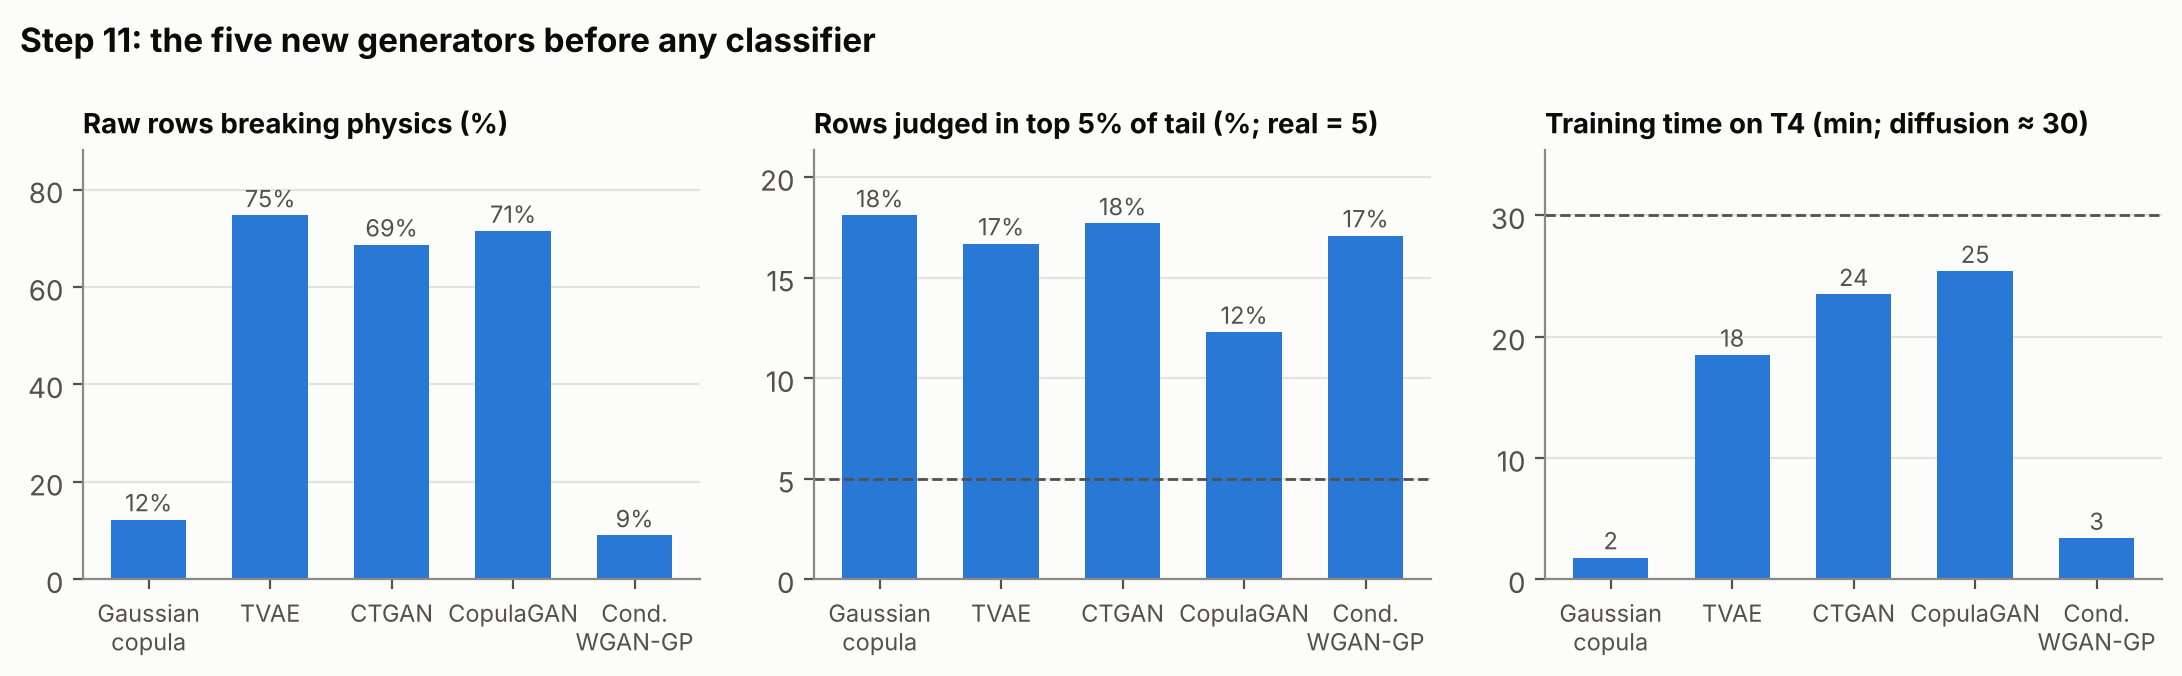
\includegraphics[width=\textwidth]{fig_generator_quality.png}
\caption{Physics violations, reach of the far tail and training time of the generators}
\label{fig:genq}
\end{figure}

The deep unconditional generators break physical rules in about 70\% of their raw rows; the conditional WGAN-GP
largely ignores the requested severity (0.25), whereas the diffusion model follows it (0.67, close to 0.78 for
real data).

\section{Comparison of Generation Methods with a Fixed Classifier}
\begin{figure}[H]
\centering
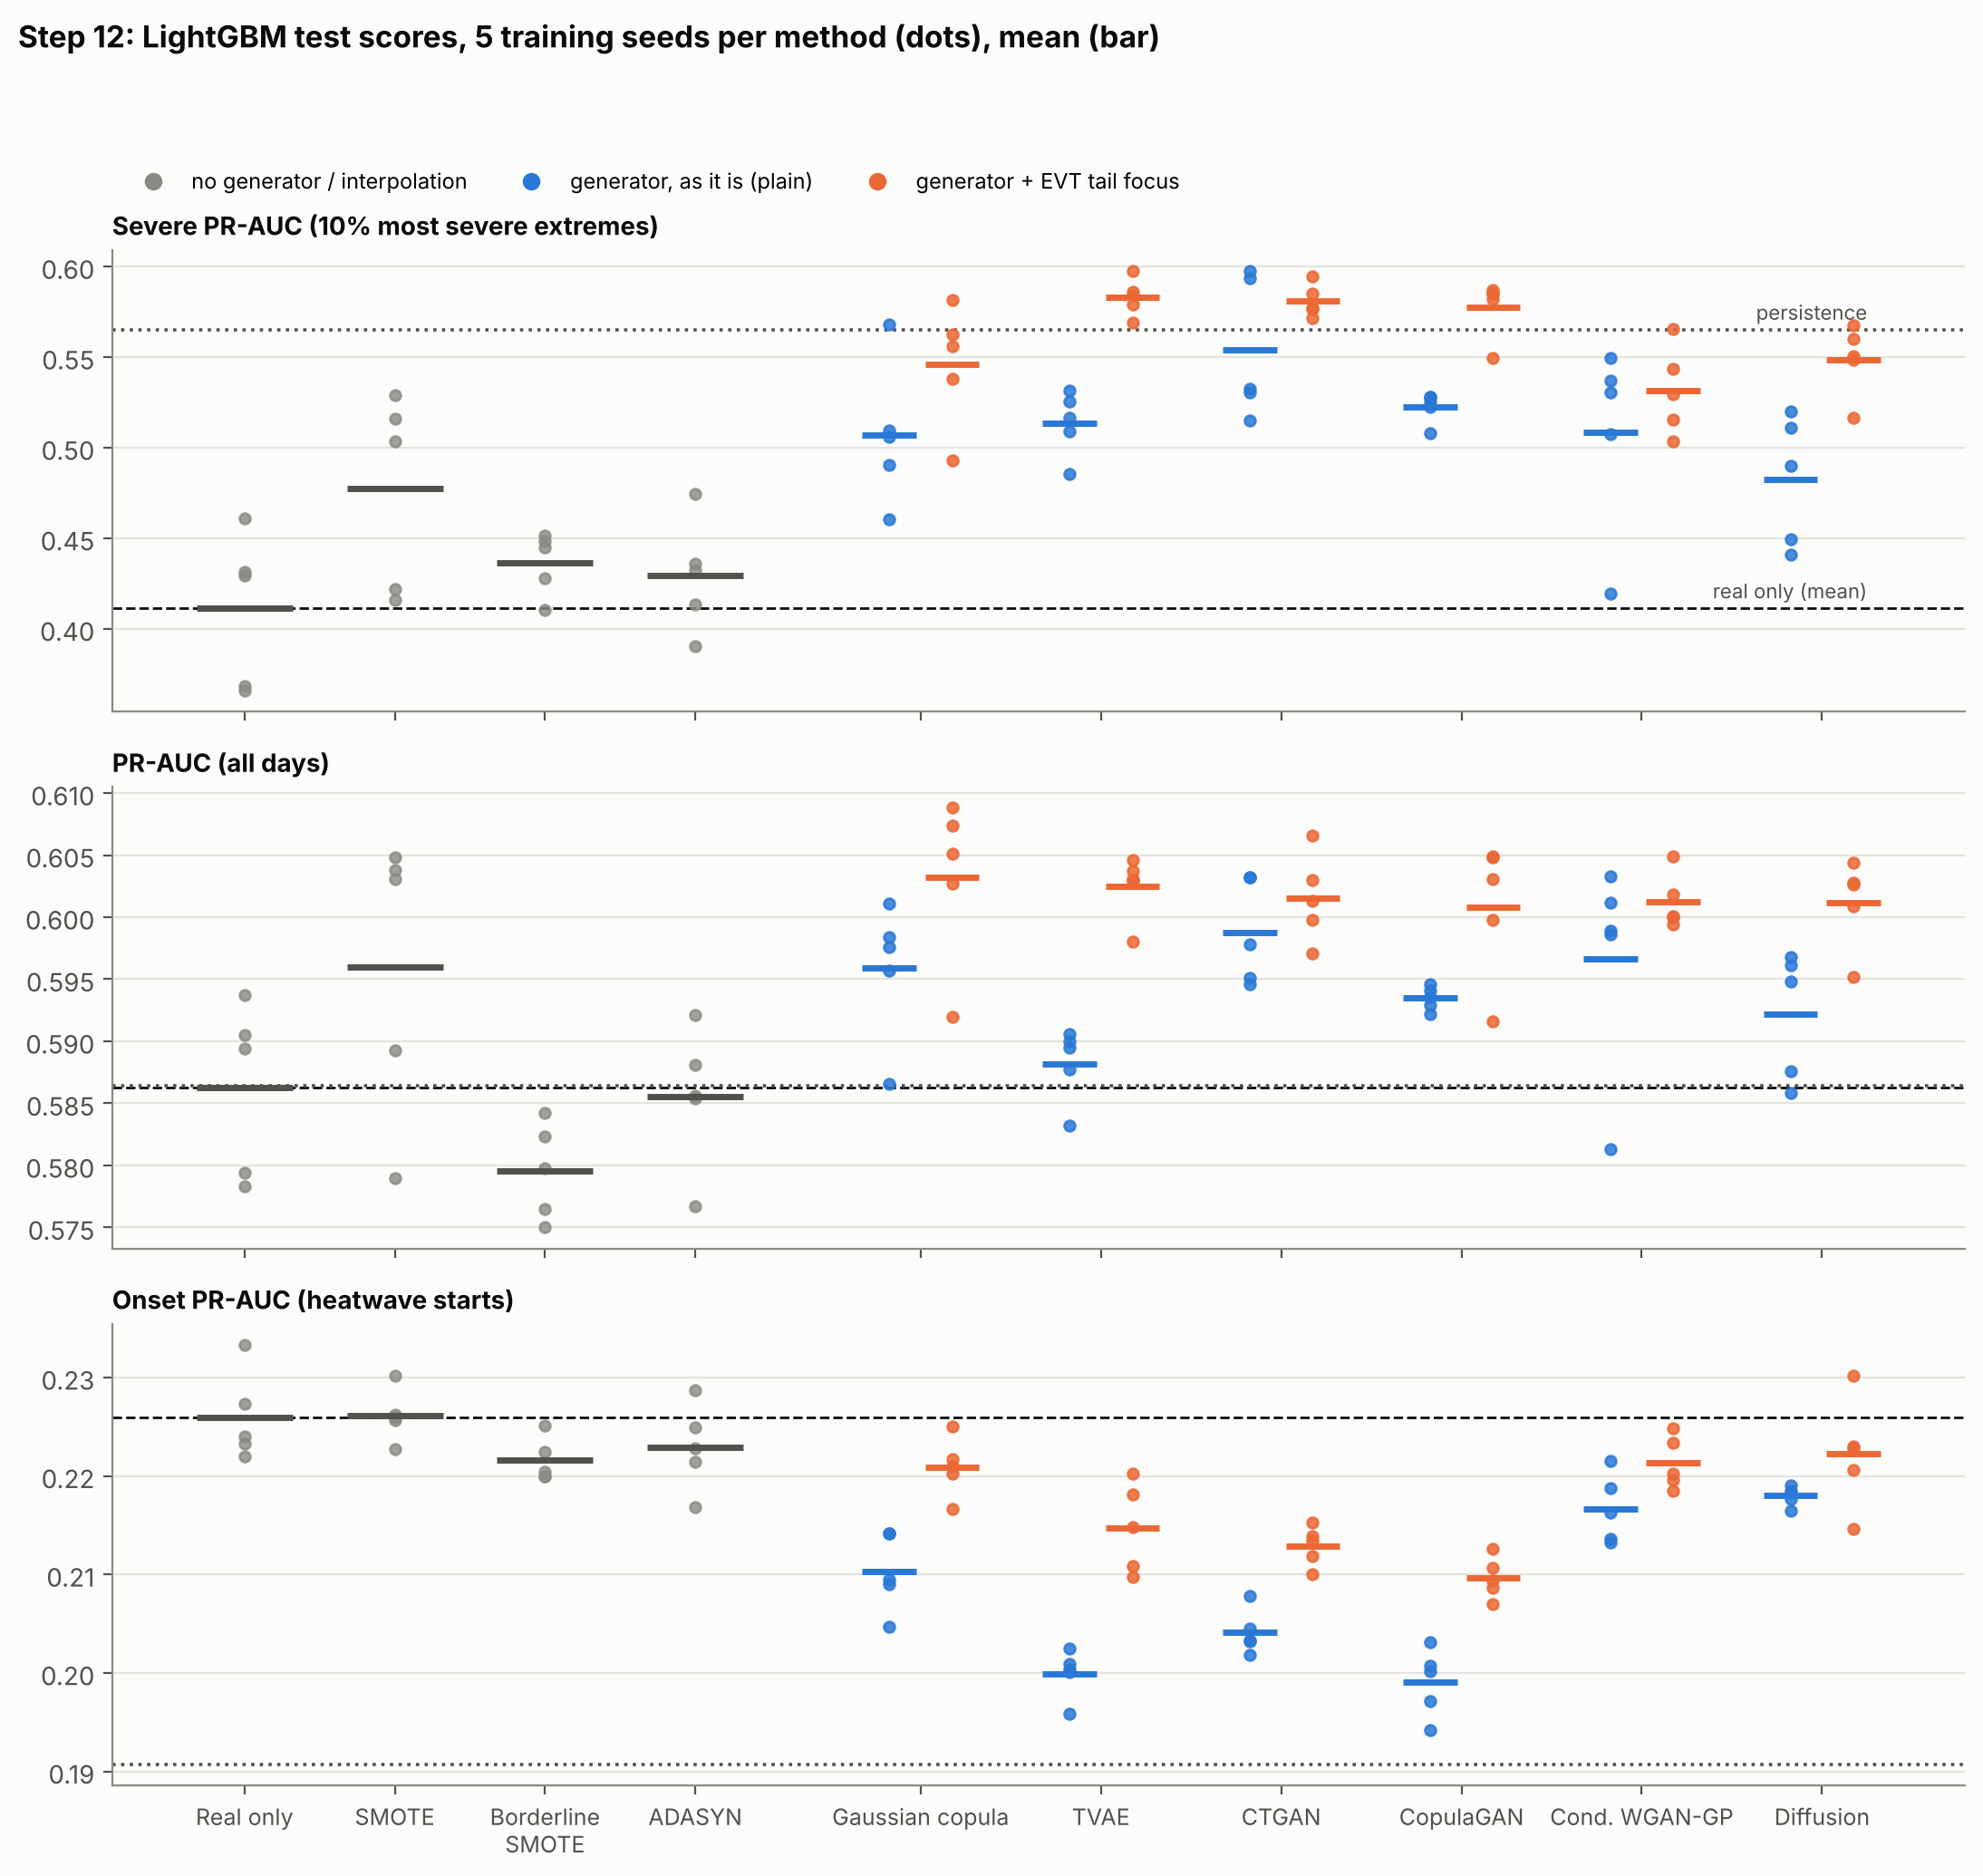
\includegraphics[width=\textwidth]{fig_step12_by_seed.png}
\caption{Test scores of every method over five training seeds (dots) and their mean (bar)}
\label{fig:step12}
\end{figure}

\begin{table}[H]
\centering
\caption{Test results over five seeds (mean $\pm$ standard deviation) and seeds that beat real data only}
\label{tab:step12}
\small
\begin{tabular}{|l|c|c|c|c|c|c|}
\hline
\textbf{Method} & \multicolumn{2}{c|}{\textbf{PR-AUC}} & \multicolumn{2}{c|}{\textbf{Onset PR-AUC}} & \multicolumn{2}{c|}{\textbf{Severe PR-AUC}}\\ \hline
Real data only & $0.586\pm0.007$ & -- & $0.226\pm0.005$ & -- & $0.411\pm0.042$ & -- \\ \hline
SMOTE & $0.596\pm0.011$ & 5/5 & $0.226\pm0.003$ & 4/5 & $0.477\pm0.054$ & 5/5 \\
Borderline-SMOTE & $0.580\pm0.004$ & 0/5 & $0.222\pm0.002$ & 0/5 & $0.437\pm0.017$ & 3/5 \\
ADASYN & $0.586\pm0.006$ & 1/5 & $0.223\pm0.004$ & 2/5 & $0.429\pm0.031$ & 4/5 \\ \hline
Gaussian copula & $0.596\pm0.006$ & 5/5 & $0.210\pm0.004$ & 0/5 & $0.507\pm0.039$ & 5/5 \\
\rowcolor{rowhl}\quad + EVT tail & $\mathbf{0.603\pm0.007}$ & 5/5 & $0.221\pm0.003$ & 1/5 & $0.546\pm0.034$ & 5/5 \\
TVAE & $0.588\pm0.003$ & 3/5 & $0.200\pm0.003$ & 0/5 & $0.514\pm0.018$ & 5/5 \\
\rowcolor{rowhl}\quad + EVT tail & $0.603\pm0.003$ & 5/5 & $0.215\pm0.005$ & 0/5 & $\mathbf{0.583\pm0.011}$ & 5/5 \\
CTGAN & $0.599\pm0.004$ & 5/5 & $0.204\pm0.002$ & 0/5 & $0.554\pm0.039$ & 5/5 \\
\rowcolor{rowhl}\quad + EVT tail & $0.602\pm0.004$ & 5/5 & $0.213\pm0.002$ & 0/5 & $0.581\pm0.009$ & 5/5 \\
CopulaGAN & $0.594\pm0.001$ & 4/5 & $0.199\pm0.004$ & 0/5 & $0.522\pm0.008$ & 5/5 \\
\rowcolor{rowhl}\quad + EVT tail & $0.601\pm0.006$ & 5/5 & $0.210\pm0.002$ & 0/5 & $0.578\pm0.016$ & 5/5 \\
Conditional WGAN-GP & $0.597\pm0.009$ & 4/5 & $0.217\pm0.004$ & 0/5 & $0.509\pm0.052$ & 4/5 \\
\rowcolor{rowhl}\quad + EVT tail & $0.601\pm0.002$ & 5/5 & $0.221\pm0.003$ & 0/5 & $0.532\pm0.024$ & 5/5 \\
Diffusion & $0.592\pm0.005$ & 3/5 & $0.218\pm0.001$ & 0/5 & $0.482\pm0.036$ & 4/5 \\
\rowcolor{rowhl}\quad + EVT tail & $0.601\pm0.004$ & 5/5 & $0.222\pm0.006$ & 1/5 & $0.549\pm0.020$ & 5/5 \\ \hline
Persistence (no model) & 0.586 & & 0.191 & & 0.565 & \\ \hline
\end{tabular}
\end{table}

\subsection{Effect of EVT tail focus}
\begin{figure}[H]
\centering
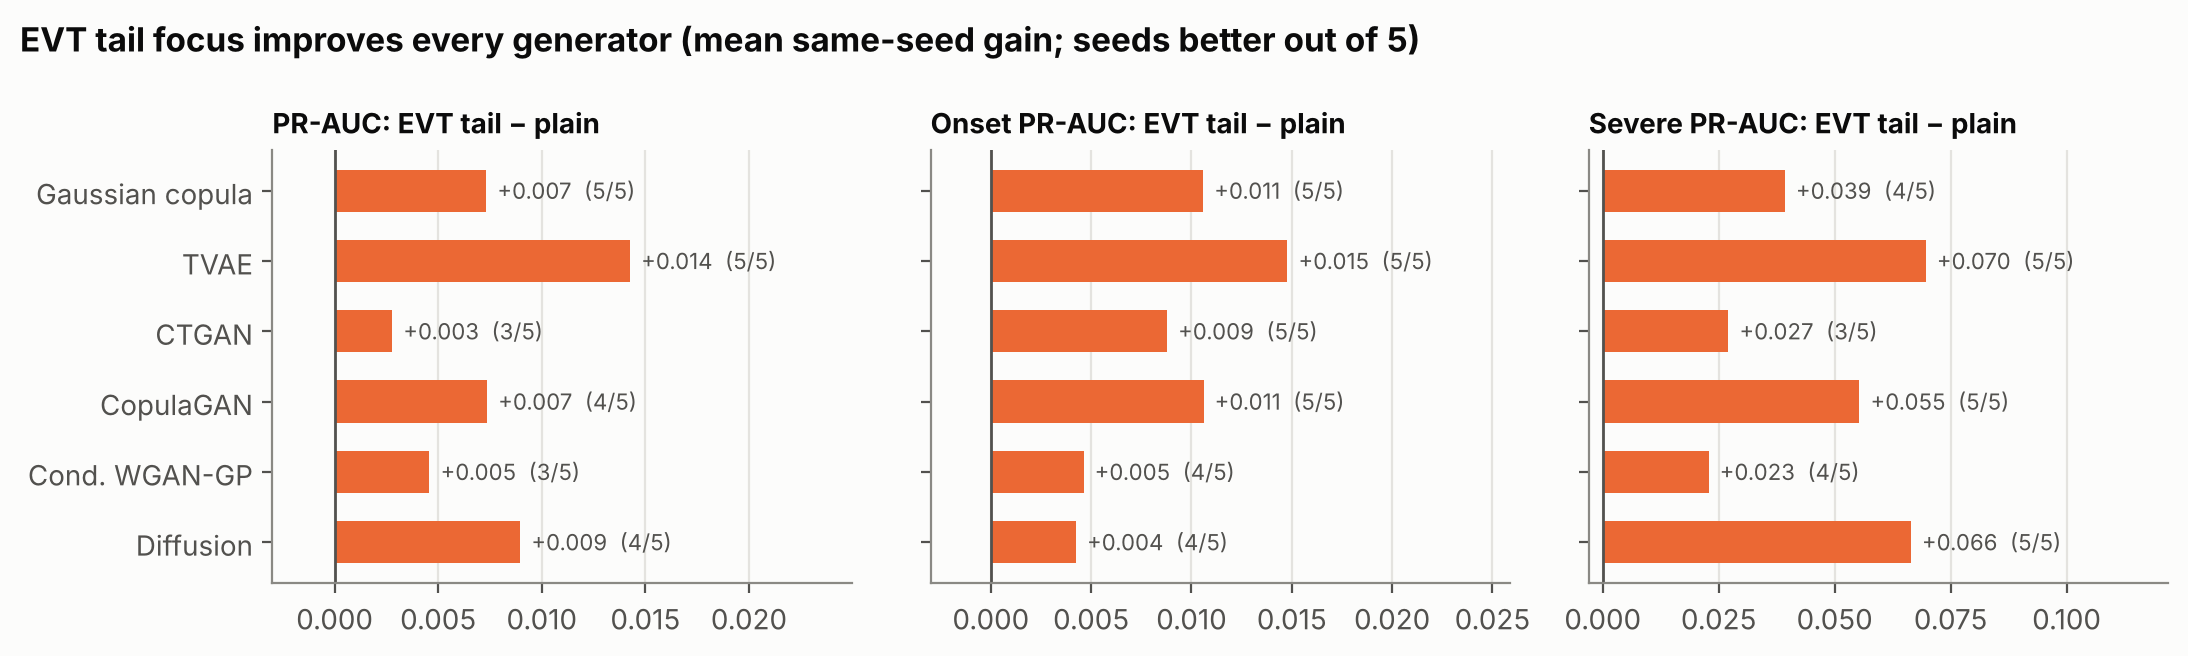
\includegraphics[width=\textwidth]{fig_evt_gain.png}
\caption{Gain of EVT tail focus over the same generator without it (mean of five same-seed differences)}
\label{fig:evtgain}
\end{figure}

Averaged over five same-seed comparisons, EVT tail focus improved every generator on all three scores
(Figure~\ref{fig:evtgain}). The most consistent gain is on heatwave onsets (better in 4--5 of 5 seeds for all six
generators); the largest gain on severe days is $+0.070$ for TVAE. All six top methods on validation are EVT-tail
versions (Table~\ref{tab:rank}).

\subsection{Seed-averaged models and ranking}
\begin{table}[H]
\centering
\caption{Seed-averaged models ordered by validation score; test scores and share of month resamples in which the model beats persistence (PR-AUC / onset / severe)}
\label{tab:rank}
\small
\begin{tabular}{|l|c|c|c|c|c|}
\hline
\textbf{Method} & \textbf{Validation} & \textbf{PR-AUC} & \textbf{Onset} & \textbf{Severe} & \textbf{Beats persistence}\\ \hline
\rowcolor{rowhl} CTGAN + EVT tail & 0.600 & 0.611 & 0.223 & \textbf{0.601} & 0.99 / 0.98 / 0.92 \\
\rowcolor{rowhl} TVAE + EVT tail & 0.600 & 0.610 & 0.220 & \textbf{0.601} & 0.97 / 0.97 / 0.90 \\
\rowcolor{rowhl} Gaussian copula + EVT tail & 0.599 & 0.608 & 0.225 & 0.558 & 0.98 / 1.00 / 0.53 \\
\rowcolor{rowhl} CopulaGAN + EVT tail & 0.595 & 0.607 & 0.214 & 0.591 & 0.96 / 0.94 / 0.79 \\
\rowcolor{rowhl} Diffusion + EVT tail & 0.594 & 0.609 & \textbf{0.228} & 0.579 & 0.97 / 1.00 / 0.73 \\
\rowcolor{rowhl} Cond.\ WGAN-GP + EVT tail & 0.581 & \textbf{0.611} & 0.226 & 0.579 & 0.99 / 0.99 / 0.70 \\
CTGAN & 0.579 & 0.609 & 0.208 & 0.595 & 0.97 / 0.83 / 0.80 \\
Gaussian copula & 0.570 & 0.606 & 0.215 & 0.555 & 0.98 / 0.96 / 0.49 \\
TVAE & 0.559 & 0.593 & 0.203 & 0.527 & 0.75 / 0.77 / 0.35 \\
SMOTE & 0.553 & 0.604 & 0.231 & 0.507 & 0.88 / 1.00 / 0.19 \\
Real data only & 0.541 & 0.599 & \textbf{0.235} & 0.441 & 0.81 / 1.00 / 0.10 \\
Diffusion & 0.541 & 0.602 & 0.224 & 0.531 & 0.90 / 0.99 / 0.26 \\ \hline
Persistence (no model) & 0.577 & 0.586 & 0.191 & 0.565 & -- \\ \hline
\end{tabular}
\end{table}

\begin{itemize}
  \item \textbf{Best methods:} CTGAN and TVAE with EVT tail focus rank first on validation, reach the highest severe
        PR-AUC on test (0.601 against 0.441 for real data only) and have the smallest seed-to-seed spread. They are
        ahead of diffusion with EVT tail focus on severe days, but not convincingly; the top EVT-tail methods are
        statistically close.
  \item \textbf{Against persistence:} CTGAN with EVT tail focus beats persistence convincingly on overall skill (99\%
        of resamples) and onset (98\%), and is ahead on severe days; real data only falls behind persistence on
        severe days.
  \item \textbf{Interpolation:} SMOTE gives a small gain on severe days; Borderline-SMOTE and ADASYN give none.
  \item \textbf{Cost:} the Gaussian copula with EVT tail focus trains in 2 minutes and ranks third on validation.
\end{itemize}

\subsection{Realism is not usefulness}
\begin{figure}[H]
\centering
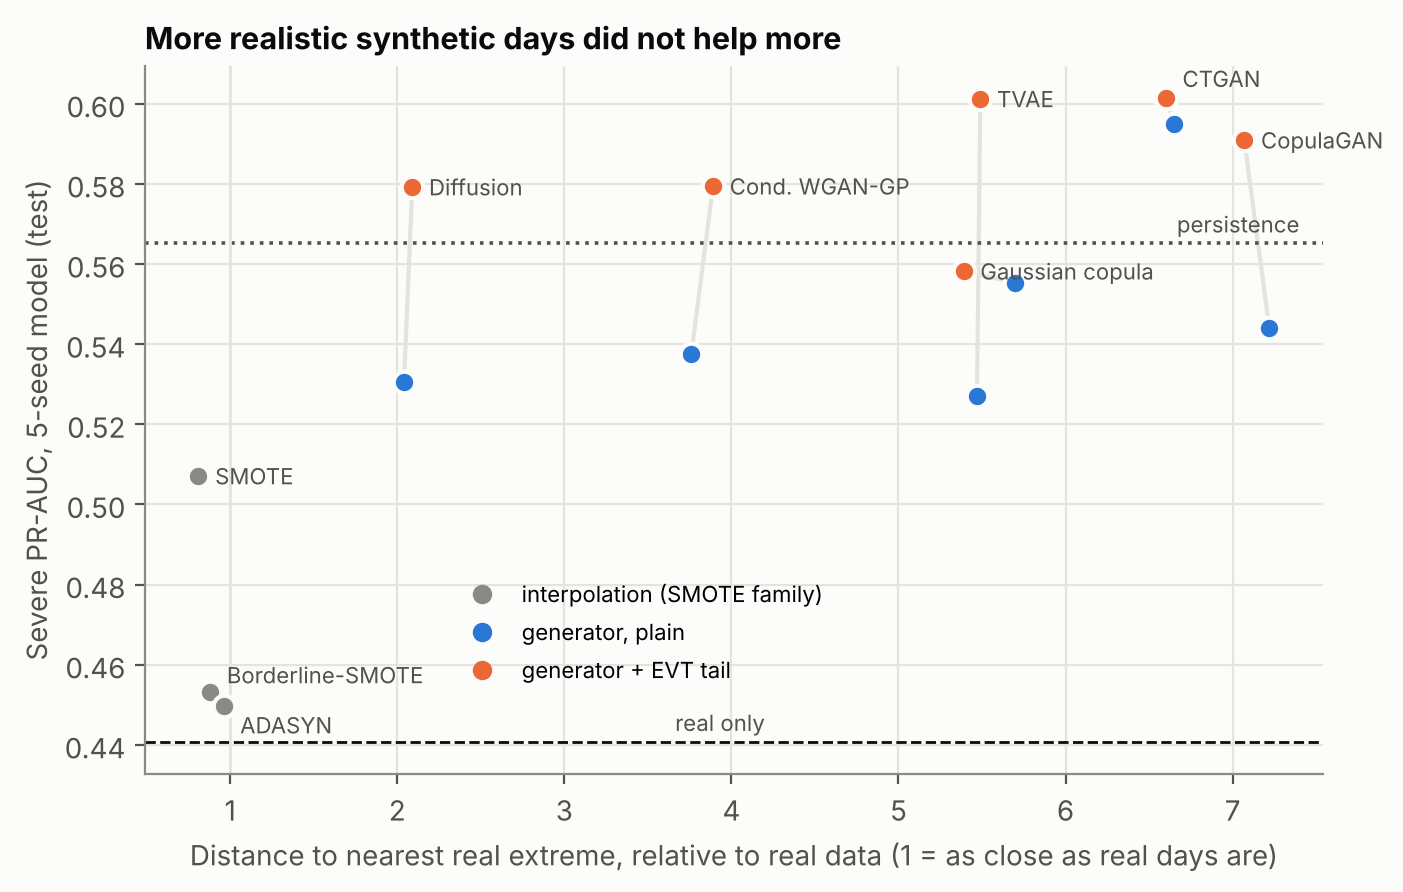
\includegraphics[width=0.85\textwidth]{fig_realism.png}
\caption{Realism of the synthetic extremes against their usefulness for the classifier}
\label{fig:realism}
\end{figure}

\begin{table}[H]
\centering
\caption{Realism of the EVT-tail sets (detection AUC: 0.5 = indistinguishable from real; closeness: 1 = as close to real days as real days are)}
\label{tab:realism}
\small
\begin{tabular}{|l|c|c|c|}
\hline
\textbf{Method} & \textbf{Detection AUC} & \textbf{Closeness} & \textbf{Severe PR-AUC}\\ \hline
SMOTE family & 0.996--0.997 & 0.81--0.96 & 0.450--0.507 \\ \hline
Diffusion + EVT tail & \textbf{0.944} & \textbf{2.09} & 0.579 \\ \hline
Cond.\ WGAN-GP + EVT tail & 0.996 & 3.89 & 0.579 \\ \hline
Gaussian copula + EVT tail & 1.000 & 5.39 & 0.558 \\ \hline
TVAE + EVT tail & 1.000 & 5.49 & 0.601 \\ \hline
CTGAN + EVT tail & 1.000 & 6.60 & 0.601 \\ \hline
CopulaGAN + EVT tail & 1.000 & 7.07 & 0.591 \\ \hline
\end{tabular}
\end{table}

The diffusion model produces by far the most realistic synthetic extremes, yet CTGAN and TVAE data---which a
classifier separates from real data perfectly and which lie five to seven times farther from real days---help the
classifier as much or more (Figure~\ref{fig:realism}, Table~\ref{tab:realism}). None of the generators copies real
rows. For a tree classifier, \emph{where} the synthetic extremes are placed matters more than whether each one is a
plausible weather situation.

\section{Control Experiment: Is a Generator Needed?}
Because unrealistic synthetic days helped as much as realistic ones, a control experiment tested the EVT emphasis
without any generator: random copies of real extremes, copies chosen with the EVT tail target, and EVT-tail training
weights with the same total emphasis.

\begin{figure}[H]
\centering
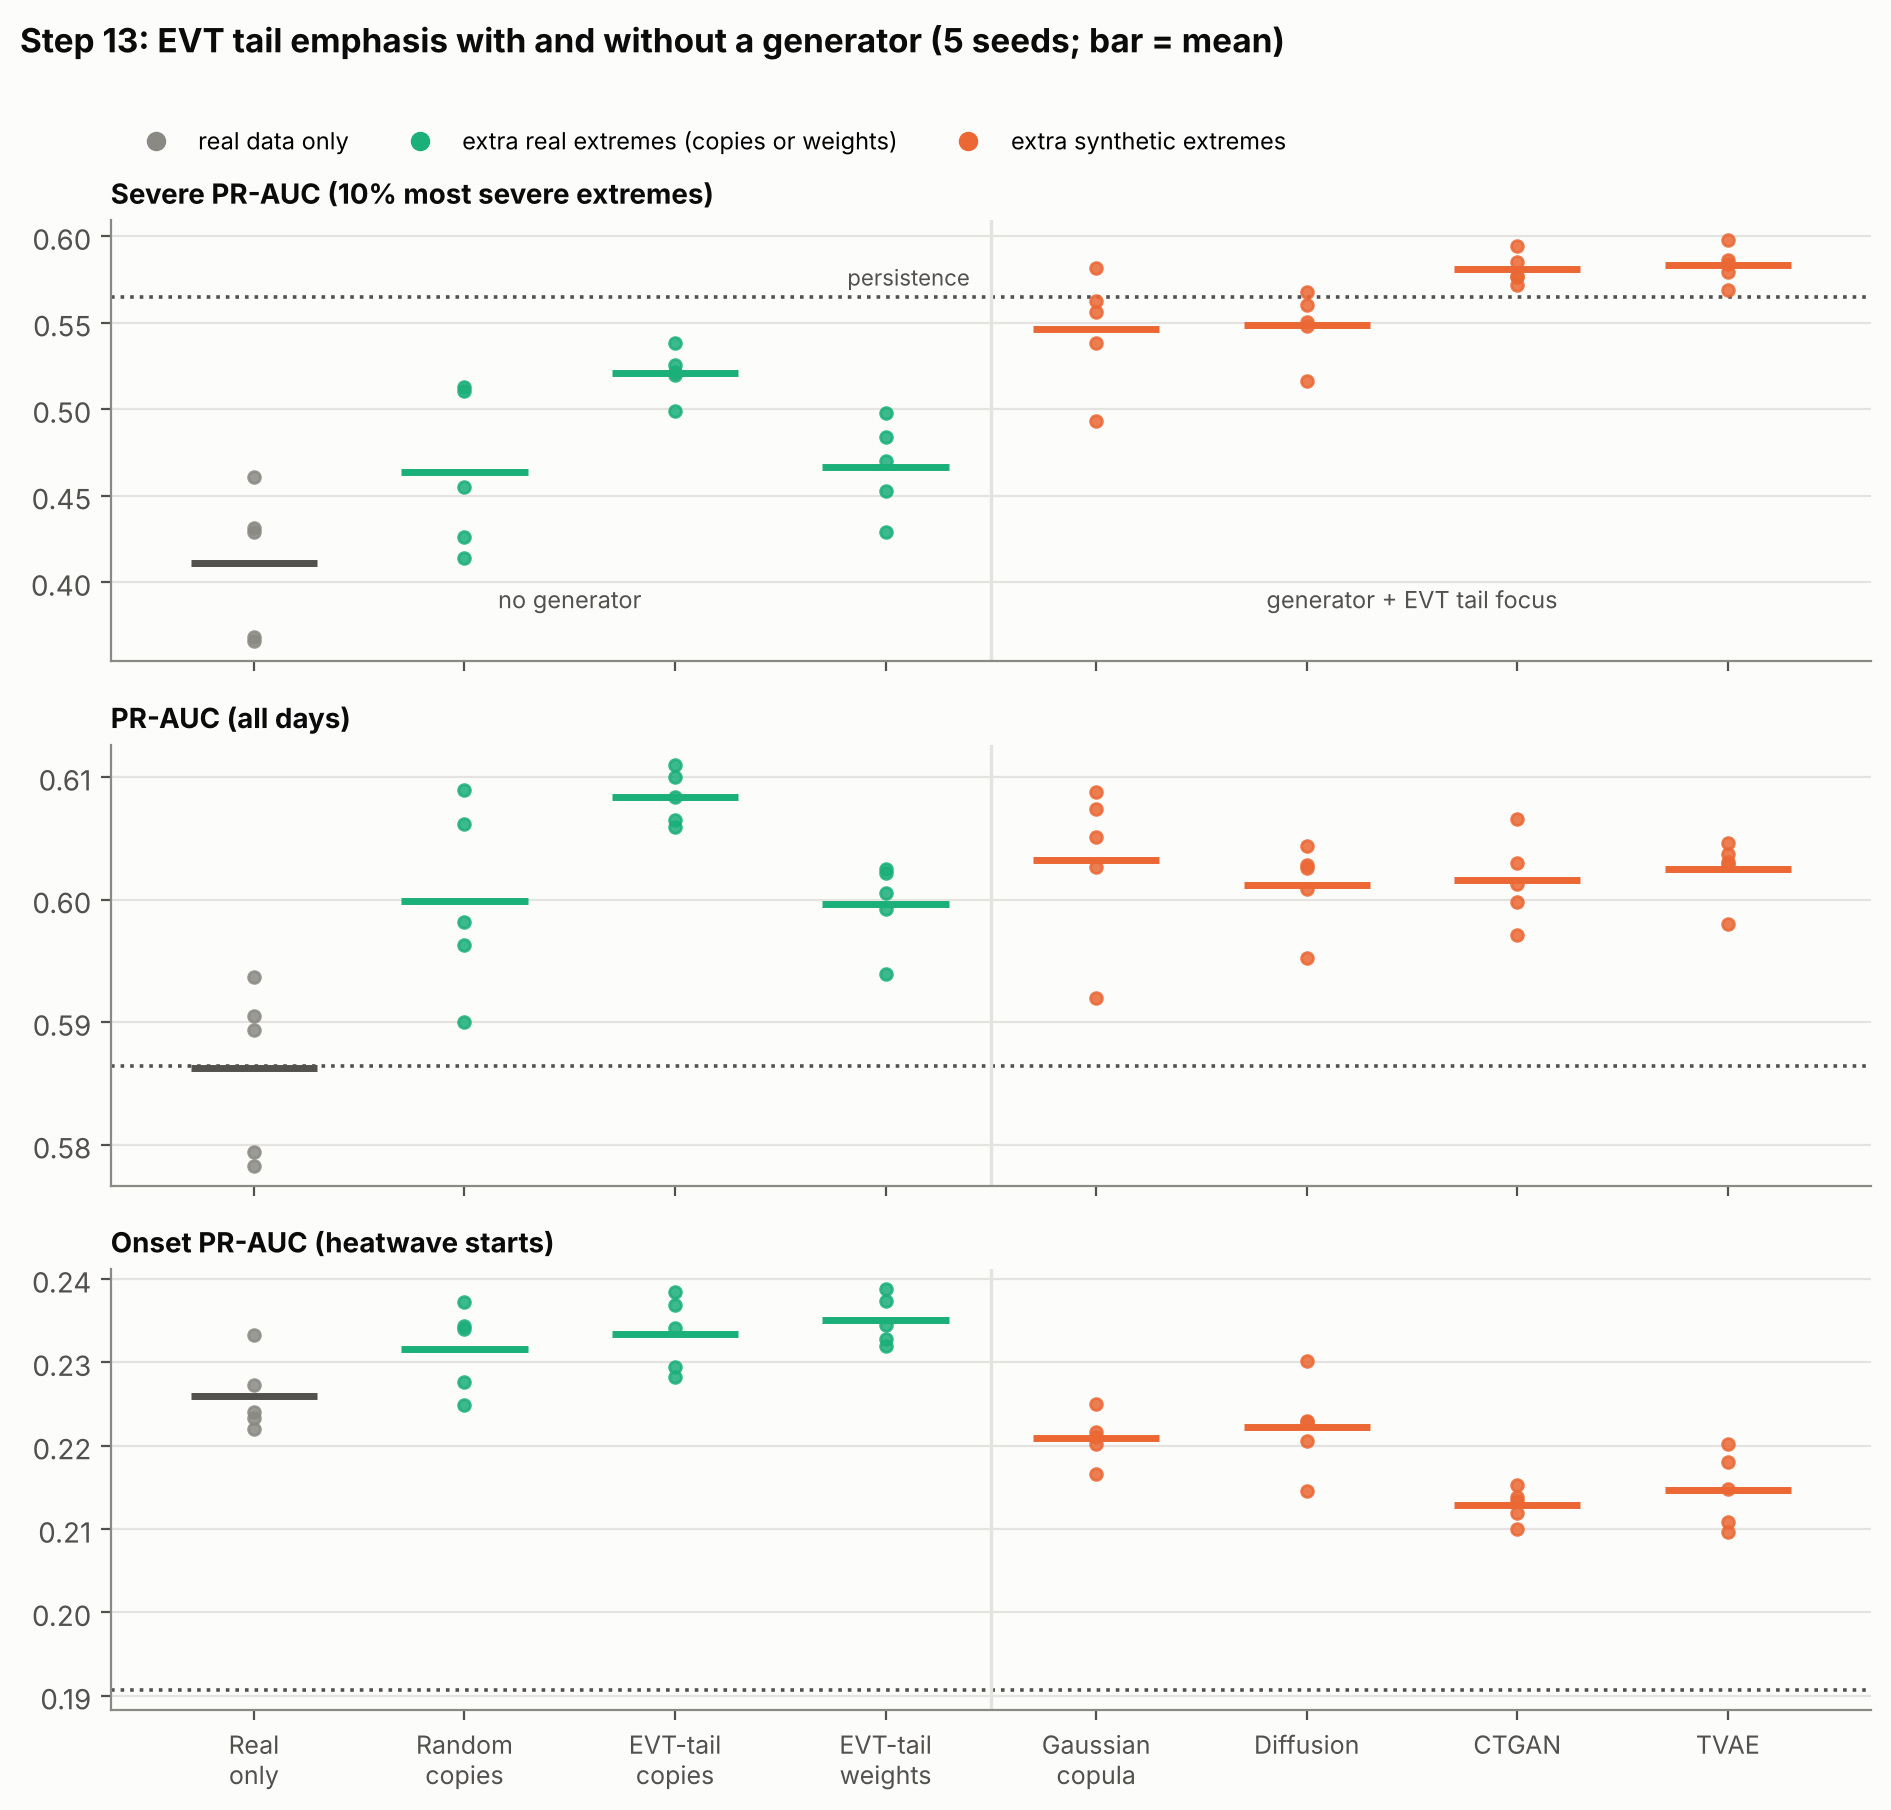
\includegraphics[width=0.9\textwidth]{fig_step13.png}
\caption{EVT tail emphasis with and without a generator: test scores of five seeds}
\label{fig:step13}
\end{figure}

\begin{table}[H]
\centering
\caption{Control experiment: test results over five seeds (mean $\pm$ standard deviation)}
\label{tab:step13}
\small
\begin{tabular}{|l|c|c|c|}
\hline
\textbf{Method} & \textbf{PR-AUC} & \textbf{Onset PR-AUC} & \textbf{Severe PR-AUC}\\ \hline
Real data only & $0.586\pm0.007$ & $0.226\pm0.005$ & $0.411\pm0.042$ \\ \hline
\rowcolor{rowhl2} Random copies of real extremes & $0.600\pm0.008$ & $0.232\pm0.005$ & $0.464\pm0.046$ \\
\rowcolor{rowhl2} EVT-tail copies of real extremes & $\mathbf{0.608\pm0.002}$ & $0.233\pm0.004$ & $0.521\pm0.014$ \\
\rowcolor{rowhl2} EVT-tail weights & $0.600\pm0.004$ & $\mathbf{0.235\pm0.003}$ & $0.467\pm0.027$ \\ \hline
CTGAN + EVT tail & $0.602\pm0.004$ & $0.213\pm0.002$ & $0.581\pm0.009$ \\
TVAE + EVT tail & $0.603\pm0.003$ & $0.215\pm0.005$ & $\mathbf{0.583\pm0.011}$ \\
Diffusion + EVT tail & $0.601\pm0.004$ & $0.222\pm0.006$ & $0.549\pm0.020$ \\ \hline
Persistence (no model) & 0.586 & 0.191 & 0.565 \\ \hline
\end{tabular}
\end{table}

\begin{table}[H]
\centering
\caption{Key comparisons: mean same-seed difference (seeds in which the first method is better)}
\label{tab:step13cmp}
\small
\begin{tabular}{|l|c|c|c|}
\hline
\textbf{Comparison} & \textbf{PR-AUC} & \textbf{Onset} & \textbf{Severe}\\ \hline
EVT-tail copies vs random copies & $+0.008$ (5/5) & $+0.002$ (4/5) & $\mathbf{+0.057}$ \textbf{(5/5)} \\ \hline
EVT-tail copies vs real data only & $+0.022$ (5/5) & $+0.008$ (5/5) & $+0.110$ (5/5) \\ \hline
CTGAN + EVT tail vs EVT-tail copies & $-0.007$ (0/5) & $-0.021$ (0/5) & $+0.060$ (5/5) \\ \hline
TVAE + EVT tail vs EVT-tail copies & $-0.006$ (0/5) & $-0.019$ (0/5) & $+0.062$ (5/5) \\ \hline
\end{tabular}
\end{table}

\begin{enumerate}
  \item \textbf{EVT works without a generator.} Copies of real extremes chosen with the EVT tail target beat random
        copies on severe days in every seed ($+0.057$).
  \item \textbf{The cheapest method is the best all-rounder.} EVT-tail copies give the highest overall PR-AUC of the
        whole study (0.608 per seed, 0.613 seed-averaged) and better onset skill than real data only, with no
        generator to train.
  \item \textbf{Generators add the far tail.} CTGAN and TVAE with EVT tail focus are better than EVT-tail copies on
        the most severe days in every seed (about $+0.06$): copies can only repeat the hottest real days, generators
        create new ones beyond them.
  \item \textbf{The price is onset skill.} The same generators are worse on heatwave onsets in every seed (about
        $-0.02$).
  \item \textbf{Copies beat weights.} With the same total emphasis, weights help less than copies on severe days,
        probably because LightGBM's minimum leaf size counts rows rather than weights.
\end{enumerate}

\section{What the Results Mean in Practice}
For the best model (CTGAN + EVT tail focus, seed-averaged), at the decision threshold chosen on validation, precision
is 0.60 and recall 0.55 on the test decade (Table~\ref{tab:practice}).

\begin{table}[H]
\centering
\caption{Warnings issued over the test decade (2016--2025, 529 cells), derived from precision and recall (approximate)}
\label{tab:practice}
\small
\begin{tabular}{|l|c|c|}
\hline
 & \textbf{Best model} & \textbf{Persistence}\\ \hline
Extreme days in the test decade & \multicolumn{2}{c|}{37{,}450} \\ \hline
Warnings issued (``extreme tomorrow'') & $\approx$34{,}300 & $\approx$40{,}800 \\ \hline
Correct warnings & $\approx$20{,}600 (55\% of extremes) & $\approx$22{,}500 (60\%) \\ \hline
False alarms & $\approx$13{,}700 (40\% of warnings) & $\approx$18{,}200 (45\%) \\ \hline
False alarms as a share of normal days & $\approx$0.7\% & $\approx$1.0\% \\ \hline
\end{tabular}
\end{table}

When the model warns, it is right about six times in ten, against two in a hundred for random guessing. The model
needs only data up to today; in operation, today's observations would come from a near-real-time source, since
ERA5-Land is published with a delay of a few days.

\section{Discussion}
\begin{itemize}
  \item \textbf{EVT decides where to add data.} A well-fitted GPD reproduces the observed severities, so sampling it
        as it is adds little; its value lies in locating the sparse upper tail and bounding how far it extends.
        Concentrating added extremes there helped every method, with or without a generator.
  \item \textbf{What a generator adds.} Generators create extremes beyond the most severe observed days, which is
        what lifts severe-day skill above persistence; copies of real days cannot. A warning system that must not
        miss the most severe heat favours a generator with EVT tail focus; an all-round forecast favours EVT-tail
        copies of real extremes.
  \item \textbf{Realism versus usefulness.} Diffusion is the right tool when synthetic weather must be physically
        plausible (for example for scenario studies); for improving a tree classifier, cheaper generators with EVT
        selection were at least as good.
  \item \textbf{Amount of synthetic data.} Synthetic extremes help in moderation; when they outnumbered real
        extremes 8.7 to 1, onset skill fell and the EVT advantage disappeared. This also explains why CTGAN hurt in
        the first comparison but helped under the final protocol.
  \item \textbf{Persistence.} Next-day heat is dominated by how hot today already is, so the absolute gain over
        persistence is modest (PR-AUC $+0.02$--$0.03$); it lies mainly in heatwave onsets and, with EVT augmentation,
        in no longer falling behind persistence on the most severe days.
  \item \textbf{Evaluation.} A one-seed result that looked convincing did not hold across seeds; rare-event results
        need several seeds, separate validation and block bootstrap tests.
\end{itemize}

\section{Limitations}
\begin{itemize}
  \item Labels and features come from a reanalysis; the severe heat days have not yet been checked against the
        three station records.
  \item Only next-day seasonal heat extremes were modelled; the test decade has twice the training rate of extremes
        and no model was adapted to this shift.
  \item EVT guides generation at sampling or selection time; it is not part of any generator's training loss.
  \item For unconditional generators, tail positions rely on a severity judge, which rates synthetic rows as more
        severe than real ones.
  \item The tail-focus setting (half from the top 20\%) was fixed by hand; one classifier family and one case study
        were tested; compute limits restricted training to half of 1981--2010.
\end{itemize}

% =============================================================================
\chapter{Conclusion and Future Work}
% =============================================================================
\section{Conclusions}
\begin{enumerate}
  \item Treating extreme heat days as the tail of the temperature distribution and modelling it with a Generalized
        Pareto Distribution of standardised excesses gives bounded, physically sensible tails and reveals a doubling
        of heat extremes and more intense winter warm spells in 2016--2025.
  \item Using EVT to concentrate added extremes in the rarest 20\% of the tail (EVT tail focus) improved every one of
        six generators under a fixed LightGBM classifier, most consistently on heatwave onsets.
  \item CTGAN and TVAE with EVT tail focus gave the best results on the most severe days (PR-AUC 0.601 against 0.441
        for real data only) and beat a strong persistence baseline on overall and onset skill.
  \item The EVT emphasis works even without a generator: EVT-tail copies of real extremes gave the best overall skill
        (0.613) at almost no cost, while generators added a further gain on the most severe days at the cost of
        onset skill.
  \item The most realistic generator was not the most useful; for a downstream classifier, where synthetic extremes
        are placed matters more than how realistic they are.
\end{enumerate}

\section{Future Work}
\begin{itemize}
  \item Validate the severe heat days against the Shimla, Sundernagar and Bhuntar station records.
  \item Choose the strength of the tail focus on validation and add a GPD term to generator training.
  \item Predict three or more days ahead, where persistence is weaker; add neighbouring cells as spatial context;
        and model the tail of tomorrow's temperature directly with extreme quantile regression~\cite{pasche2024eqrn}.
  \item Test the framework on public imbalanced data sets beyond weather.
\end{itemize}

% =============================================================================
%  TIMELINE / OUTCOMES
% =============================================================================
\clearpage
\leftchapter{Timeline/ Outcomes}
% Edit the weeks below to match your actual schedule: \gA / \gB = filled cell, empty = nothing.
\newcommand{\gB}{\cellcolor{ganttB}}
\newcommand{\gA}{\cellcolor{ganttA}}
\begin{table}[H]
\centering
\small
\setlength{\tabcolsep}{4pt}
\begin{tabular}{|p{5.6cm}|*{8}{p{0.62cm}|}}
\hline
\rowcolor{gray!55}
\textcolor{white}{\textbf{Outcomes}} & \multicolumn{4}{c|}{\textcolor{white}{\textbf{October 2026}}} & \multicolumn{4}{c|}{\textcolor{white}{\textbf{November 2026}}}\\ \hline
 & \centering W1 & \centering W2 & \centering W3 & \centering W4 & \centering W1 & \centering W2 & \centering W3 & \centering\arraybackslash W4 \\ \hline
Data collection and verification & \gA & \gA & & & & & & \\ \hline
Literature review & & \gA & \gA & & & & & \\ \hline
Labels, features, EVT analysis & & & \gA & \gA & & & & \\ \hline
Baselines and GAN experiments & & & & \gA & & & & \\ \hline
Diffusion model and 5-seed evaluation & & & & \gA & \gB & & & \\ \hline
Generator comparison (fixed LightGBM) & & & & & & \gB & & \\ \hline
Control experiment & & & & & & \gB & & \\ \hline
Report and presentation & & & & & \gB & & \gB & \gB \\ \hline
\end{tabular}
\caption{Project timeline}
\label{tab:timeline}
\end{table}

\textbf{Outcomes:} a verified 45-year data set of seasonal heat extremes for 529 grid cells; an extreme value model of
the heat tail; an EVT-guided conditional diffusion model and conditional WGAN-GP; a fair comparison of ten data
generation methods under a fixed classifier; and open, reproducible code that runs on free cloud resources:\\
\url{https://github.com/Divyansh-jain2/Major_Technical_Project}

% =============================================================================
%  REFERENCES
% =============================================================================
\renewcommand{\bibname}{References:}
{\titleformat{name=\chapter,numberless}[block]{\normalfont\bfseries\fontsize{22}{26}\selectfont\filright}{}{0pt}{}
\begin{thebibliography}{99}
\addcontentsline{toc}{chapter}{References}
\setlength{\itemsep}{2pt}
\small
\bibitem{coles2001} S. Coles, \reflink{https://doi.org/10.1007/978-1-4471-3675-0}{An Introduction to Statistical Modeling of Extreme Values}, Springer, 2001.
\bibitem{pickands1975} J. Pickands, \reflink{https://doi.org/10.1214/aos/1176343003}{Statistical inference using extreme order statistics}, Annals of Statistics 3 (1975) 119--131.
\bibitem{balkema1974} A. A. Balkema and L. de Haan, \reflink{https://doi.org/10.1214/aop/1176996548}{Residual life time at great age}, Annals of Probability 2 (1974) 792--804.
\bibitem{chawla2002smote} N. V. Chawla, K. W. Bowyer, L. O. Hall and W. P. Kegelmeyer, \reflink{https://doi.org/10.1613/jair.953}{SMOTE: Synthetic minority over-sampling technique}, Journal of Artificial Intelligence Research 16 (2002) 321--357.
\bibitem{han2005borderline} H. Han, W.-Y. Wang and B.-H. Mao, \reflink{https://doi.org/10.1007/11538059_91}{Borderline-SMOTE: A new over-sampling method in imbalanced data sets learning}, International Conference on Intelligent Computing, 2005.
\bibitem{he2008adasyn} H. He, Y. Bai, E. A. Garcia and S. Li, \reflink{https://doi.org/10.1109/IJCNN.2008.4633969}{ADASYN: Adaptive synthetic sampling approach for imbalanced learning}, IEEE International Joint Conference on Neural Networks, 2008.
\bibitem{elor2022smote} Y. Elor and H. Averbuch-Elor, \reflink{https://arxiv.org/abs/2201.08528}{To SMOTE, or not to SMOTE?}, arXiv:2201.08528, 2022.
\bibitem{goodfellow2014gan} I. Goodfellow et al., \reflink{https://arxiv.org/abs/1406.2661}{Generative adversarial nets}, Advances in Neural Information Processing Systems, 2014.
\bibitem{gulrajani2017wgangp} I. Gulrajani, F. Ahmed, M. Arjovsky, V. Dumoulin and A. Courville, \reflink{https://arxiv.org/abs/1704.00028}{Improved training of Wasserstein GANs}, Advances in Neural Information Processing Systems, 2017.
\bibitem{xu2019ctgan} L. Xu, M. Skoularidou, A. Cuesta-Infante and K. Veeramachaneni, \reflink{https://arxiv.org/abs/1907.00503}{Modeling tabular data using conditional GAN}, Advances in Neural Information Processing Systems, 2019.
\bibitem{kingma2014vae} D. P. Kingma and M. Welling, \reflink{https://arxiv.org/abs/1312.6114}{Auto-encoding variational Bayes}, International Conference on Learning Representations, 2014.
\bibitem{patki2016sdv} N. Patki, R. Wedge and K. Veeramachaneni, \reflink{https://doi.org/10.1109/DSAA.2016.49}{The Synthetic Data Vault}, IEEE International Conference on Data Science and Advanced Analytics, 2016.
\bibitem{ho2020ddpm} J. Ho, A. Jain and P. Abbeel, \reflink{https://arxiv.org/abs/2006.11239}{Denoising diffusion probabilistic models}, Advances in Neural Information Processing Systems, 2020.
\bibitem{nichol2021improved} A. Nichol and P. Dhariwal, \reflink{https://arxiv.org/abs/2102.09672}{Improved denoising diffusion probabilistic models}, International Conference on Machine Learning, 2021.
\bibitem{song2021ddim} J. Song, C. Meng and S. Ermon, \reflink{https://arxiv.org/abs/2010.02502}{Denoising diffusion implicit models}, International Conference on Learning Representations, 2021.
\bibitem{ho2022cfg} J. Ho and T. Salimans, \reflink{https://arxiv.org/abs/2207.12598}{Classifier-free diffusion guidance}, arXiv:2207.12598, 2022.
\bibitem{kotelnikov2023tabddpm} A. Kotelnikov, D. Baranchuk, I. Rubachev and A. Babenko, \reflink{https://arxiv.org/abs/2209.15421}{TabDDPM: Modelling tabular data with diffusion models}, International Conference on Machine Learning, 2023.
\bibitem{dsouza2025overlap} A. D'souza, Swetha M and S. Sarawagi, \reflink{https://arxiv.org/abs/2412.15657}{Synthetic tabular data generation for imbalanced classification: The surprising effectiveness of an overlap class}, AAAI Conference on Artificial Intelligence, 2025.
\bibitem{bhatia2021exgan} S. Bhatia, A. Jain and B. Hooi, \reflink{https://arxiv.org/abs/2009.08454}{ExGAN: Adversarial generation of extreme samples}, AAAI Conference on Artificial Intelligence, 2021.
\bibitem{boulaguiem2022evtgan} Y. Boulaguiem, J. Zscheischler, E. Vignotto, K. van der Wiel and S. Engelke, \reflink{https://arxiv.org/abs/2111.00267}{Modeling and simulating spatial extremes by combining extreme value theory with generative adversarial networks}, Environmental Data Science 1 (2022) e5.
\bibitem{pandey2025heavy} K. Pandey et al., Heavy-tailed diffusion models, International Conference on Learning Representations, 2025.
\bibitem{jalalzai2018extreme} H. Jalalzai, S. Cl\'emen\c{c}on and A. Sabourin, On binary classification in extreme regions, Advances in Neural Information Processing Systems, 2018.
\bibitem{lopezgomez2023heat} I. Lopez-Gomez, A. McGovern, S. Agrawal and J. Hickey, \reflink{https://arxiv.org/abs/2205.10972}{Global extreme heat forecasting using neural weather models}, Artificial Intelligence for the Earth Systems, 2023.
\bibitem{zhang2025records} Z. Zhang, E. Fischer, J. Zscheischler and S. Engelke, \reflink{https://arxiv.org/abs/2508.15724}{Numerical models outperform AI weather forecasts of record-breaking extremes}, arXiv:2508.15724, 2025.
\bibitem{bhan_imd} S. C. Bhan, \reflink{https://heathealth.info/wp-content/uploads/Poster_SC-Bhan_FGFHH-Subhash-Bhan.pdf}{Heat wave forecasting and early warning services of the India Meteorological Department} (poster), Global Heat Health Information Network.
\bibitem{ke2017lightgbm} G. Ke et al., LightGBM: A highly efficient gradient boosting decision tree, Advances in Neural Information Processing Systems, 2017.
\bibitem{munoz2021era5land} J. Mu\~noz-Sabater et al., \reflink{https://doi.org/10.5194/essd-13-4349-2021}{ERA5-Land: A state-of-the-art global reanalysis dataset for land applications}, Earth System Science Data 13 (2021) 4349--4383.
\bibitem{farr2007srtm} T. G. Farr et al., \reflink{https://doi.org/10.1029/2005RG000183}{The Shuttle Radar Topography Mission}, Reviews of Geophysics 45 (2007) RG2004.
\bibitem{pasche2024eqrn} O. C. Pasche and S. Engelke, \reflink{https://arxiv.org/abs/2208.07590}{Neural networks for extreme quantile regression with an application to forecasting of flood risk}, Annals of Applied Statistics 18 (2024).
\end{thebibliography}}

\end{document}
